 \documentclass[11pt,a4paper]{article}
\usepackage[latin1]{inputenc}
\usepackage{cite}
\usepackage{lmodern}
\usepackage{lipsum}
\usepackage[export]{adjustbox}
\usepackage{amsmath}
\usepackage{amsfonts}
\usepackage{amssymb}
\usepackage{graphicx}
\usepackage{subcaption}
\usepackage{marginnote}
\usepackage{verbatim}
\usepackage{color}   %May be necessary if you want to color links
\usepackage{hyperref}
\hypersetup{
    colorlinks=true, %set true if you want colored links
    linktoc=all,     %set to all if you want both sections and subsections linked
    linkcolor=blue,  %choose some color if you want links to stand out
}
\usepackage[bottom]{footmisc}
\usepackage[top=1.5cm, bottom=3cm, outer=2cm, inner=2cm, heightrounded, marginparwidth=3cm, marginparsep=3cm]{geometry}
\usepackage{listings}
\usepackage{color}

\definecolor{dkgreen}{rgb}{0,0.6,0}
\definecolor{gray}{rgb}{0.5,0.5,0.5}
\definecolor{mauve}{rgb}{0.58,0,0.82}

\lstset{frame=tb,
	language=Python,
	aboveskip=3mm,
	belowskip=3mm,
	showstringspaces=false,
	columns=flexible,
	basicstyle={\small\ttfamily},
	numbers=none,
	numberstyle=\tiny\color{gray},
	keywordstyle=\color{blue},
	commentstyle=\color{dkgreen},
	stringstyle=\color{mauve},
	breaklines=true,
	breakatwhitespace=true,
	tabsize=3
}
\author{Rachana(PH15B007)\\Guide:Prof.Arul Lakshminarayan}
\title{Project Report}

\begin{document}

\maketitle
\newpage
	\tableofcontents 
	\pagebreak
	
		 \section{Entanglement Dynamics in Kicked Ising Model }
		 
		 \subsection{Defining the Hamiltonian}
		 
	      Consider a 1-D spin chain with interactions only along the x-axis, and a pulsed magnetic field along z-axis which acts on all spins at once.  
		 
		 Hamiltonian for kicked Ising model with periodic boundary conditions is given by:
		 \begin{equation}\label{key}
		 H(t)= \sum_{j=1}^{L}\sigma_{j}^{x} \sigma_{j+1}^{x} + \sum_{k=-\infty}^{\infty}\delta(k-\dfrac{t}{T})\sum_{j=1}^{L}\sigma_{j}^{z}
		 \end{equation}
		 Here $T$ is the time period after which the kicks are applied to the Ising chain. 
		
Deriving time evolution operator for Floquet system:

The Schr\"{o}dinger equation for this kicked Ising model is given by (let $\sum_{j=1}^{L}\sigma_{j}^{x} \sigma_{j+1}^{x}  = H_{0} $ and $\sum_{j=1}^{L}\sigma_{j}^{z} = H_{1}$),

\begin{equation}
i \hbar \dfrac{\partial}{\partial t}|\psi\rangle = H_{0}|\psi\rangle + H_{1} \delta_{T}(t) |\psi\rangle
\end{equation}

Here $\delta_{T}(t) =  \sum_{k=-\infty}^{\infty}\delta(k-\dfrac{t}{T})$. In the time interval between two consecutive kicks, only $H_{0}$ contributes to the unitary operator. So, therefore we define:
\begin{equation}
U_{after} = \exp(-iH_{0}T/\hbar)
\end{equation}

Here $U_{after}$ is the unitary operator that acts between consecutive kicks. Now, in order to find the unitary evolution operator at the time of the kick, we integrate the Schr\"{o}dinger equation over an infinetisimal time about $t = T $. This eliminates the $H_{0}$ part and we will be left with:
\begin{equation}
i\hbar \dfrac{\partial}{\partial t} |\psi\rangle = H_{1}\delta_{T}(t) |\psi\rangle
\end{equation}

Solving by integrating over an infinitesimal time duration $\epsilon$, we get (and setting $\hbar = 1$):
\begin{align}
i \log(\dfrac{|\psi(T+\epsilon)\rangle}{|\psi(T-\epsilon)\rangle}) &= \int_{T-\epsilon}^{T+\epsilon} H_{1}\delta_{T}(t)\\
|\psi(T+\epsilon)\rangle &= \exp(-iH_{1}T)|\psi(T-\epsilon)\rangle 
\end{align}
This gives the time evolution operator at the time of kick to be:
\begin{equation}
U_{kick} = \exp(-iH_{1}T)
\end{equation}
		 
		In this study, we consider the evolution with the time period $\dfrac{\pi}{4}$\cite{PhysRevA.91.022318}. Hence the overall unitary operator driving the system for one time period would be:
		 
		 \begin{equation}
		 U = U_{after}U_{kick} = \exp(-i\dfrac{\pi}{4}\sum_{j=1}^{L}\sigma_{j}^{x} \sigma_{j+1}^{x})  \exp(-i\dfrac{\pi}{4}\sum_{j=1}^{L}\sigma_{j}^{z})
		 \end{equation}
		 
		 Making the Hamiltonian aperiodic by incorporating the idea from \cite{PhysRevX.7.031034}, where the $n^{th}$ kick occurring at time $t= nT$ is shifted to $t = nT + \tau_{n}dt$ where $\tau_{n} = \pm 1$, and we explore the behaviour of the system for various sequences of $\tau_{n}$'s in the form for example, $\tau = \{1,-1,1,-1,-1,1,\cdots\}$. The Dirac train in the Hamiltonian for this following case takes the form:
		 \begin{equation}
		 \delta_{T}(t) =  \sum_{k=-\infty}^{\infty}\delta(k-\dfrac{t-\tau_{n}dt}{T})
		 \end{equation}

In this case, the time interval between consecutive kicks becomes $T + (\tau_{n+1}-\tau_{n})dt$. So, this changes the time evolution operators in the following ways:
\begin{align}
U_{after} &= \exp(-i
		 (\dfrac{\pi}{4}+(\tau_{n+1}-\tau_{n})\text{dt})\sum_{j=1}^{L}\sigma_{j}^{x} \sigma_{j+1}^{x})\\
		 U_{kick} &=  \exp(-i(\dfrac{\pi}{4})\sum_{j=1}^{L}\sigma_{j}^{z}) 
\end{align}

		With this, the overall time evolution operator acting the $n^{th}$ time takes the form:
		 \begin{equation}
		 U_{n} = \exp[-i
		 \dfrac{\pi}{4}(1+(\tau_{n+1}-\tau_{n})\dfrac{\text{dt}}{\pi/4})\sum_{j=1}^{L}\sigma_{j}^{x} \sigma_{j+1}^{x}]  \exp[-i\dfrac{\pi}{4}\sum_{j=1}^{L}\sigma_{j}^{z}]
		 \end{equation}
		 
		Since $\tau_{n}= \pm 1$, we define a sequence $\mu$ such that $\mu_{n} = (\tau_{n+1}-\tau_{n})$. So, $\mu\, \epsilon \,\{2,0,-2\}$. For the cases where $\dfrac{\text{dt}}{\pi/4} \ll 1$, the evolution of the subsystem entanglement entropy with number of kicks resembles that of the evolution with $ \text{dt} = 0 $.\\
		

		
	Now	we explore the special case where dt $= \dfrac{\pi}{8}$. 
	\begin{align}
	 U_{after} &=\exp(-i
		 (\dfrac{\pi}{4}+\mu_{n} \dfrac{\pi}{8})\sum_{j=1}^{L}\sigma_{j}^{x} \sigma_{j+1}^{x})\\
		  U_{after} &= \begin{cases}
		  				\exp(-i\dfrac{\pi}{4}\sum_{j=1}^{L}\sigma_{j}^{x} \sigma_{j+1}^{x}) & \mu_{n} = 0\\
		  				1 & \mu_{n} = -2\\
		  				\exp(-i\dfrac{\pi}{2}\sum_{j=1}^{L}\sigma_{j}^{x} \sigma_{j+1}^{x}) & \mu_{n} = 2
		  				\end{cases} \\
	 \end{align} 
		
	Notice the case $\mu_{n} = 2$. Here, 
\begin{align}
	\exp(-i\dfrac{\pi}{2}\sum_{j=1}^{L}\sigma_{j}^{x} \sigma_{j+1}^{x}) &= \prod_{j=1}^{L}\exp(-i\dfrac{\pi}{2}\sigma_{j}^{x} \sigma_{j+1}^{x})\\
	&= \prod_{j=1}^L (-i\sigma_{j}^{x} \sigma_{j+1}^{x})\\
	&= (-i)^L 
\end{align}	
		
		
So the entanglement properties of the system is not affected whenever $\mu_{n}\, \epsilon \, \{2,-2\} $.


\begin{figure}[h!]
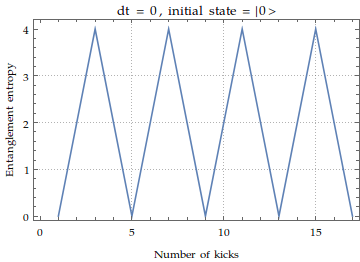
\includegraphics[scale=0.8,center]{dt0.png}
\caption{Starting with the initial state $|0\rangle$ in a 8-spin chain, entanglement entropy of the subsystem consisting of first 4 spins is being plotted with time for dt = 0 }
\label{normal}
\end{figure}

\begin{comment}
\begin{figure}[h]
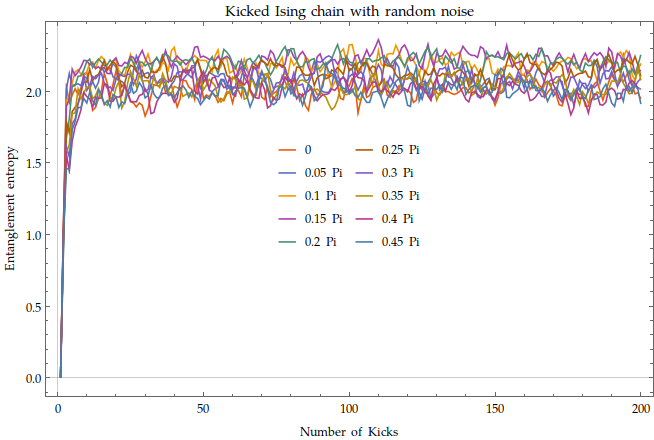
\includegraphics[scale=0.8,center]{Cnoise8.png}
\caption{Plot of entanglement entropy for the aperiodic hamiltonian with random noise for different initial states}
\end{figure}
\end{comment}

\begin{figure}[h]
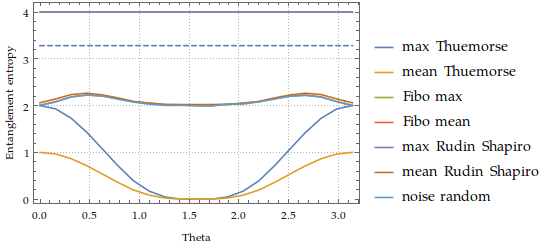
\includegraphics[scale=0.8,center]{correct.png}
\caption{Plot of entanglement entropy for the aperiodic hamiltonian with different sequences for different initial states}
\end{figure}
\begin{figure}[h]
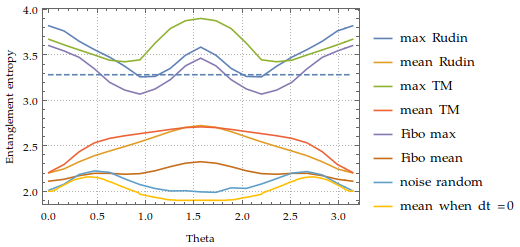
\includegraphics[scale=0.8,center]{ECCall.png}
\caption{Plot of entanglement entropy for the aperiodic hamiltonian with sequences itself and not the first difference present in the Unitary operator for different initial states}
\end{figure}

\begin{comment}

\subsubsection{Analysis with Thue Morse Sequence}
 Consider the Thue-Morse sequence given by $\tau_{tm} = \{1,-1,-1,1,-1,1,1,-1,\\-1,1,1,-1,1,-1,-1,\cdots \}$. And $\mu_{tm} = \{-2, 0, 2, -2, 2, 0, -2, 0, 2, 0, -2, 2, -2, 0, 2, -2, 2, \cdots\} $. Consider the initial state to be the $|+\rangle_{\otimes L}$ state (eigenstate of the interaction term) where $|+\rangle = \dfrac{|1\rangle+|0\rangle}{\sqrt{2}}$ and $|1\rangle$ and $|0\rangle$ are the eigenvectors of $\sigma^z$ with eigen values -1 and 1 respectively. 

\begin{comment}
\begin{figure}[h]
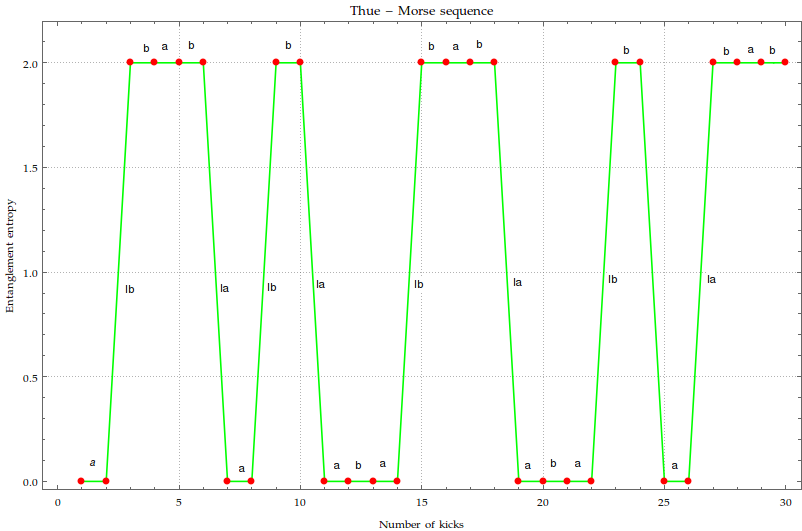
\includegraphics[scale=0.5,center]{tmcorrect.png}
\caption{Starting with the initial state $|0\rangle$ in a 8-spin chain, entanglement entropy of the subsystem consisting of first 4 spins is being ploteed with the subsequent the operation of evolution operators modelled according to the Thue Morse sequence.}
\label{thuemorse1}
\end{figure}
\end{comment}





The state after $n$ kicks is given by:
\begin{equation}
|\psi(n)\rangle = U_{n}U_{n-1}\cdots U_{2}U_{1}|\psi(0)\rangle
\end{equation}

\begin{comment}
Let us investigate how the action of $U_{1},U_{2},\cdots$ affects the entanglement properties.

\begin{align}
\tau_{1} = 1 ,\, \mu_{1} = -2 \, &: \, U_{1} = \exp(-i\dfrac{3\pi}{8}\sum_{j=1}^L\sigma_{j}^z) \doteq  A = a\\
\tau_{2} = -1 ,\, \mu_{2} = 0 \, &: \, U_{2} = \exp(-i\dfrac{\pi}{4}\sum_{j}\sigma_{j+1}^x\sigma_{j}^x)\exp(-i\dfrac{\pi}{8}\sum_{j=1}^L\sigma_{j}^z) \doteq B = Ib\\
\tau_{3} = -1 ,\, \mu_{3} = 2 \, &: \, U_{3} =(-i)^L \exp(-i\dfrac{\pi}{8}\sum_{j=1}^L\sigma_{j}^z) \doteq C = b\\
\tau_{4} = 1 ,\, \mu_{4} = -2 \, &: \, U_{4} = \exp(-i\dfrac{3\pi}{8}\sum_{j=1}^L\sigma_{j}^z)\doteq A = a \\
\tau_{5} = -1 ,\, \mu_{5} = 2 \, &: \, U_{5} =(-i)^L \exp(-i\dfrac{\pi}{8}\sum_{j=1}^L\sigma_{j}^z) \doteq C = b \\
\tau_{6} = 1 ,\, \mu_{6} = 0 \, &: \, U_{6} = \exp(-i\dfrac{\pi}{4}\sum_{j}\sigma_{j+1}^x\sigma_{j}^x)\exp(-i\dfrac{3\pi}{8}\sum_{j=1}^L\sigma_{j}^z) \doteq D =Ia 
\end{align}  

Notice that, $ab = ba = \prod_{j=1}^L \sigma_{j}^z$

\end{comment}

A nice property of the Thue Morse sequence is that it is cube-free, from this we can conclude that in the sequence $\mu\, \epsilon\, \{-2,0,2\}$, there appears no occurances of consecutive $0$'s. This results in the entanglement entropy of the subsystem oscillating between only 2 values one of which is $0$ as can be seen in Figure:\ref{thuemorse1}. Taking the case where the initial state of the system is $|+\rangle_{\otimes L}$, the subsystem entanglement entropy stays at 0 for all times. 


\end{comment}

		 
		 \subsubsection{Evolution with different initial states}
		 Consider the initial state to be.
		 \begin{equation}
		 |\psi\rangle = \prod_{\otimes L}(\cos\dfrac{\theta}{2}|0\rangle + e^{i\phi} \sin\dfrac{\theta}{2}|1\rangle )
		 \end{equation}
		 
		 Since the hamiltonian does not have a $\sigma^y$ term, varying $\phi$ will not affect the dynamics of the system. Now studying the dynamics of $|\psi(n)\rangle$ (where $n$ is the number of kicks) for different values of $\theta$ (for 2 spin system). \\
		 
		 For this system, the Unitary operator with periodic boundary condition would be:
		 \begin{align}
		 U &= \exp(-i\dfrac{\pi}{2}\sigma_{1}^x\sigma_{2}^x)\exp(-i\dfrac{\pi}{4}(\sigma_{1}^z+\sigma_{2}^z))\\
		 &= -i\sigma_{1}^x\sigma_{2}^x + \dfrac{1-i(\sigma_{1}^z+\sigma_{2}^z)}{\sqrt{2}}
		 \end{align}
		
		 \textbf{Case 1 : }
		 
		 $\theta = 0$
		 \begin{align}
		|\psi(0)\rangle &= |00\rangle\\
		|\psi(1)\rangle & = \exp(-i\dfrac{\pi}{4}\sigma_{1}^{x} \sigma_{2}^{x})  \exp(-i\dfrac{\pi}{4}\sum_{j=1}^{2}\sigma_{j}^{z})|00\rangle \\
		&= \dfrac{1}{2\sqrt{2}}(I -i\sigma_{1}^{x} \sigma_{2}^{x})(I-i\sigma_{1}^{z})(I-i\sigma_{2}^{z})|00\rangle	\\
		&= \dfrac{1}{2\sqrt{2}}(1-i)^2 (|00\rangle + i |11\rangle)
		\end{align}
		
		\begin{align}
		|\psi(2)\rangle = \dfrac{1}{2\sqrt{2}}((1-i)^4 (|00\rangle + i |11\rangle) + i(1-i)^2 (1+i)^2 (|00\rangle + i|11\rangle) 
		\end{align}
		
\begin{figure}
\centering
\begin{subfigure}[c]{.85\linewidth}
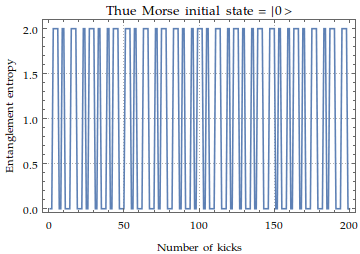
\includegraphics[scale=0.7]{Ectm.png}
\end{subfigure}
\begin{subfigure}[c]{.85\linewidth}
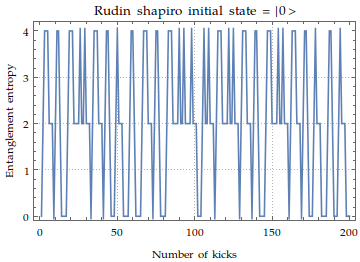
\includegraphics[scale=0.7]{Ecrudin.png}
\end{subfigure}
\begin{subfigure}[c]{.85\linewidth}
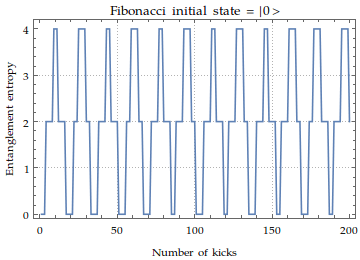
\includegraphics[scale=0.7]{Ecfibo.png}
\end{subfigure}
\caption{The Unitary operator contains the first difference of the above given sequces and the system was let to evolve with dt = pi/8}
\end{figure}

\begin{figure}
\centering
\begin{subfigure}[c]{.85\linewidth}
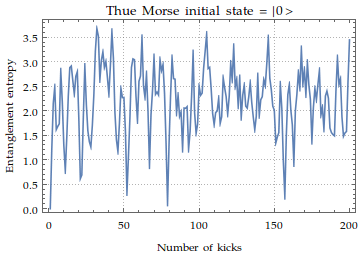
\includegraphics[scale=0.7]{ECCtm.png}
\end{subfigure}
\begin{subfigure}[c]{.85\linewidth}
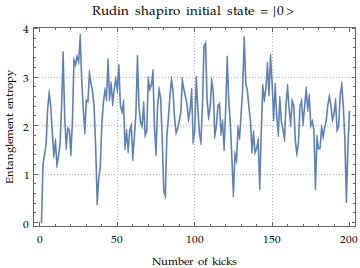
\includegraphics[scale=0.7]{ECCrudin.png}
\end{subfigure}
\begin{subfigure}[c]{.85\linewidth}
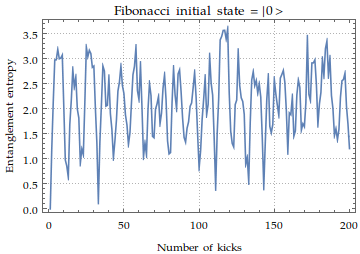
\includegraphics[scale=0.7]{ECCfibo.png}
\end{subfigure}
\caption{The Unitary operator contains the sequence itself intead of the fisrt difference of the above given sequces and the system was let to evolve with dt = pi/8}
\end{figure}
	
		 

\begin{comment}
\begin{figure}[h!]
\centering
\begin{subfigure}[c]{.85\linewidth}
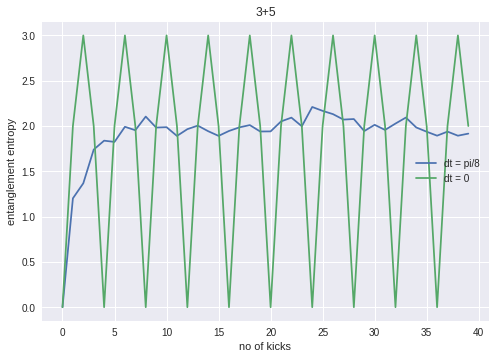
\includegraphics[scale=0.7]{3_5_0_0.png}
\caption{Starting with the initial state $|+\rangle$ in a 8-spin chain, entanglement entropy of the subsystem consisting of first 3 spins is being plotted with time for dt = 0 and dt = pi/8}
\end{subfigure}
\begin{subfigure}[c]{.85\linewidth}
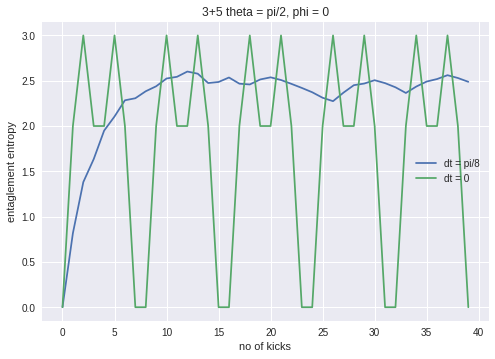
\includegraphics[scale=0.7]{3_5_piby2_0_8.png}
\caption{Starting with the initial state $|0\rangle$ in a 8-spin chain, entanglement entropy of the subsystem consisting of first 3 spins is being plotted with time for dt = 0 and dt = pi/8}
\end{subfigure}
\end{figure}
\begin{figure}
\centering
\begin{subfigure}[c]{.85\linewidth}
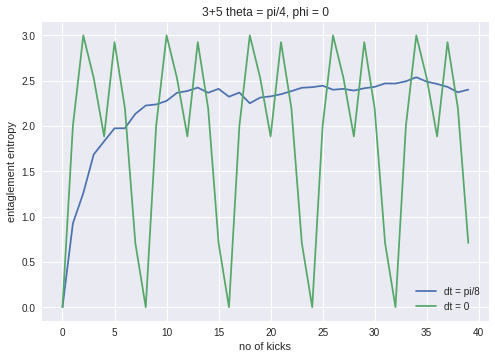
\includegraphics[scale=0.7]{3_5_piby4_0_8.png}
\end{subfigure}
\begin{subfigure}[c]{.85\linewidth}
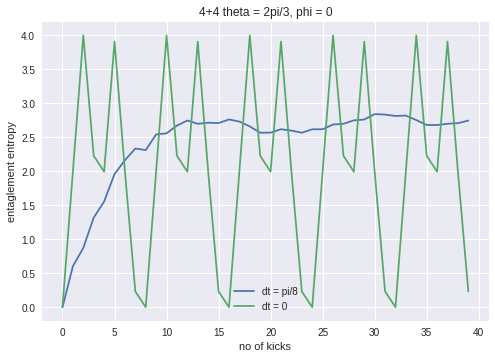
\includegraphics[scale=0.7]{4_4_2piby3_0_8.png}
\end{subfigure}
\begin{subfigure}[c]{.85\linewidth}
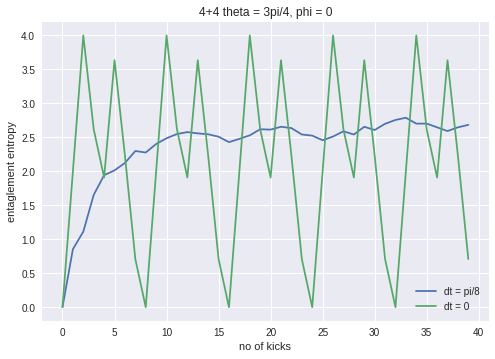
\includegraphics[scale=0.7]{4_4_3piby4_0_8.png}
\end{subfigure}
\end{figure}
\begin{figure}
\centering
\begin{subfigure}[c]{.85\linewidth}
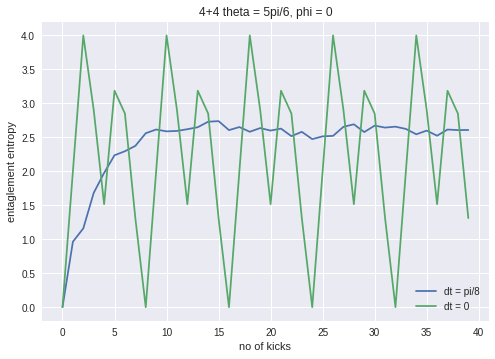
\includegraphics[scale=0.7]{4_4_5piby6_0_8.png}
\end{subfigure}
\begin{subfigure}[c]{.85\linewidth}
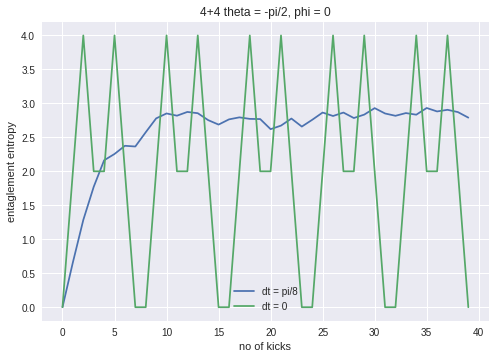
\includegraphics[scale=0.7]{4_4_minuspiby2.png}
\end{subfigure}
\end{figure}
\end{comment}

		 \begin{comment}
		 
		 \begin{align}
		 \exp(-i\dfrac{\pi}{4}\sum_{j=1}^{L}\sigma_{j}^{z})& = \prod_{j=1}^{L}\exp(-i\dfrac{\pi}{4}\sigma_{j}^{z})\\
		 & = \prod_{j=1}^{L}\dfrac{(I_{j}-i\sigma_{j}^{z})}{\sqrt{2}}\\
		 \exp(-i\dfrac{\pi}{4}\sum_{j=1}^{L}\sigma_{j}^{z})|j_{1}j_{2}j_{3}j_{4}j_{5}j_{6}j_{7}j_{8}\rangle & = \prod_{\otimes j}\dfrac{1-(-1)^j i}{\sqrt{2^L}}|j\rangle
		 \end{align}
		 
		 \begin{align}
		 \exp(-i\dfrac{\pi}{4}\sum_{j=1}^{L-1}\sigma_{j}^{x} \sigma_{j+1}^{x}) & = \prod_{j=1}^{L-1}\exp(-i\dfrac{\pi}{4}\sigma_{j}^{x} \sigma_{j+1}^{x})\\
		 & = \prod_{j=1}^{L-1}\dfrac{(I_{j}I_{j+1}-i\sigma_{j}^{x} \sigma_{j+1}^{x})}{\sqrt{2}}\\
		  \exp(-i\dfrac{\pi}{4}\sum_{j=1}^{L-1}\sigma_{j}^{x} \sigma_{j+1}^{x})\prod_{\otimes j}\dfrac{1-(-1)^j i}{\sqrt{2^L}}|j\rangle & = 
		 \end{align}
		 
		
		 
		\end{comment} 
		 
	
	\begin{comment}
	\begin{figure}[h!]
        
        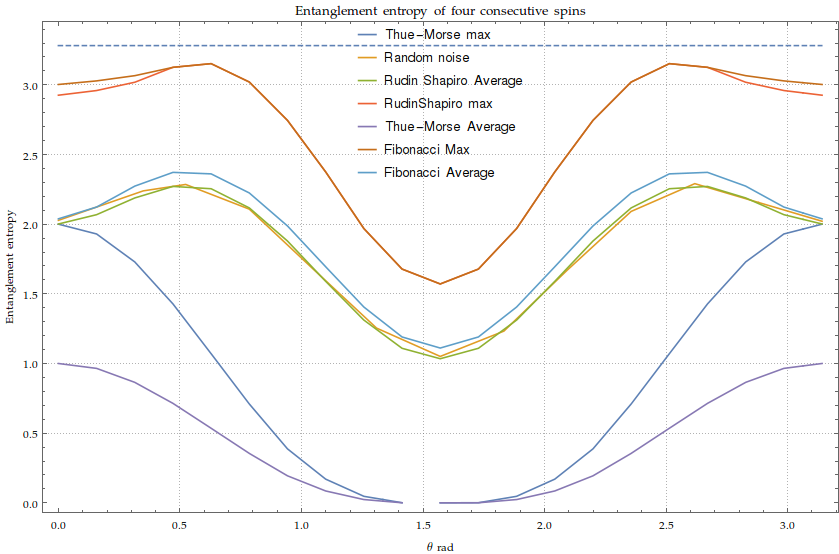
\includegraphics[width=1.1\textwidth]{saturation_plots.png} % first figure itself
        \caption{The dashed line is the average entropy of a totally random subsystem\cite{PhysRevLett.71.1291}. In the above figure Ising chain with 8 spins (periodic boundary conditions) is considered and entanglement is calculated between the two halves (4+4) spins}
		 \label{saturationplots}
    
        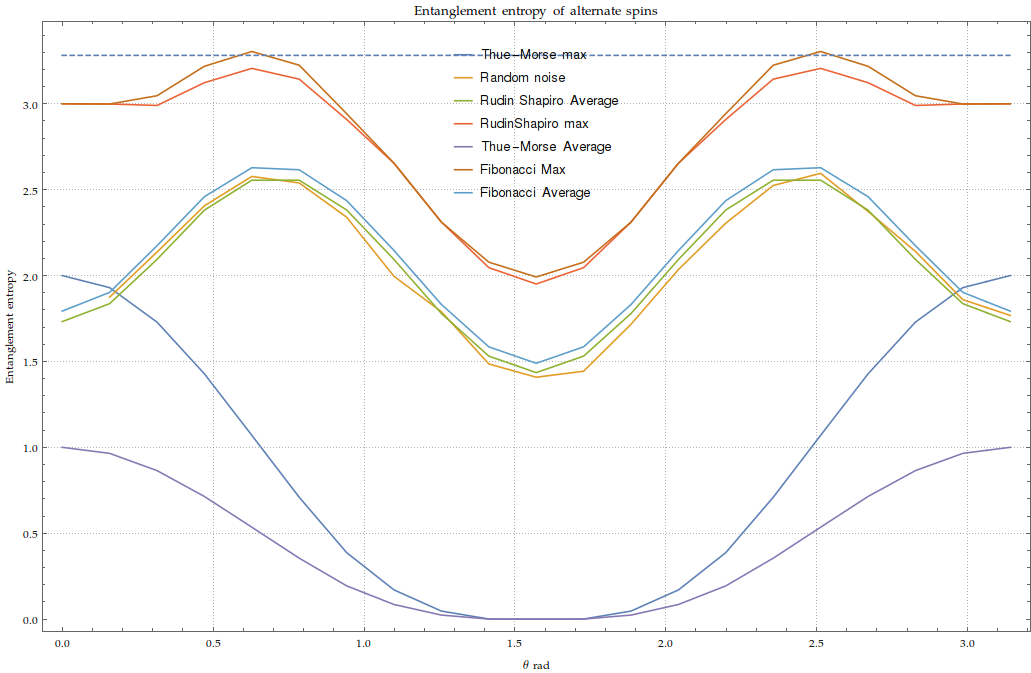
\includegraphics[width=1.1\textwidth]{alternateentropy.png} % second figure itself
        \caption{Comb entanglement entropy.}
		 \label{altsaturationplots}
  
\end{figure}
		
		  
\begin{figure}[h!]
\centering
\begin{subfigure}[c]{.65\linewidth}
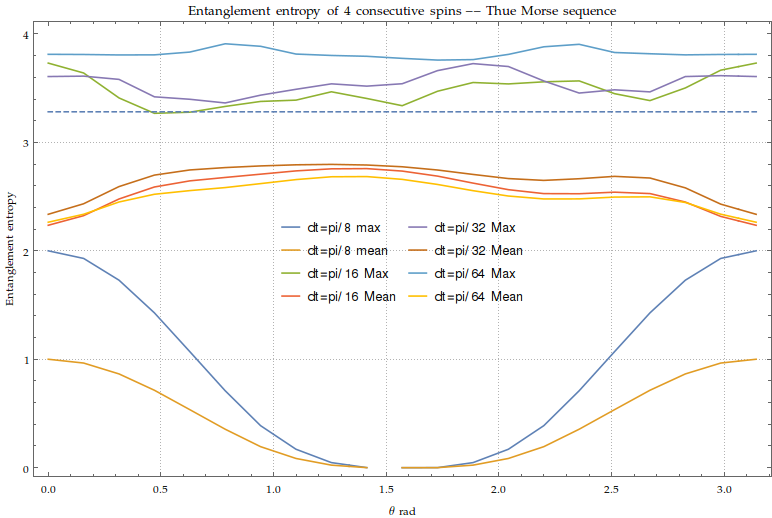
\includegraphics[width=\linewidth]{tm.png}
\caption{Thue Morse}
\end{subfigure}

\begin{subfigure}[c]{.65\linewidth}
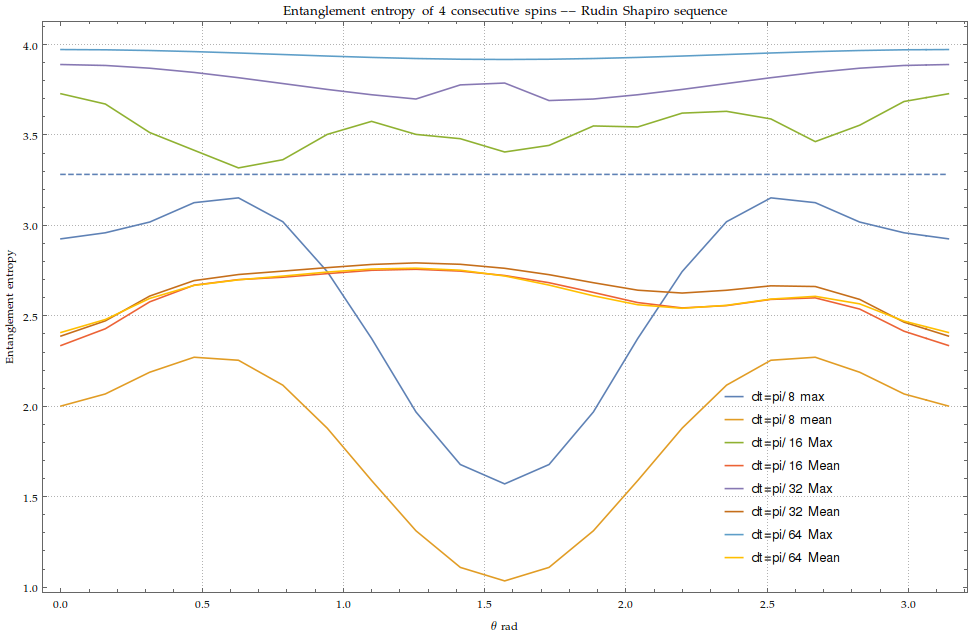
\includegraphics[width=\linewidth]{rd.png}
\caption{Rudin Shapiro}
\end{subfigure}

\begin{subfigure}[c]{.65\linewidth}
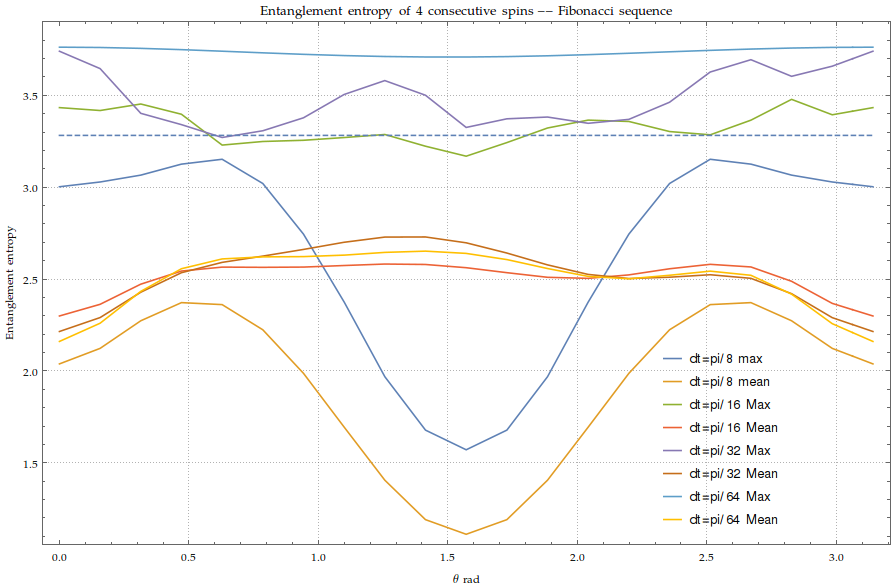
\includegraphics[width=\linewidth]{fibo.png}
\caption{Fibonacci}
\end{subfigure}
\caption{Plot of entanglement entropy for the aperiodic hamiltonian versus different initial states (theta) and different values of dt.}
\end{figure} 

\begin{figure}[h!]
		 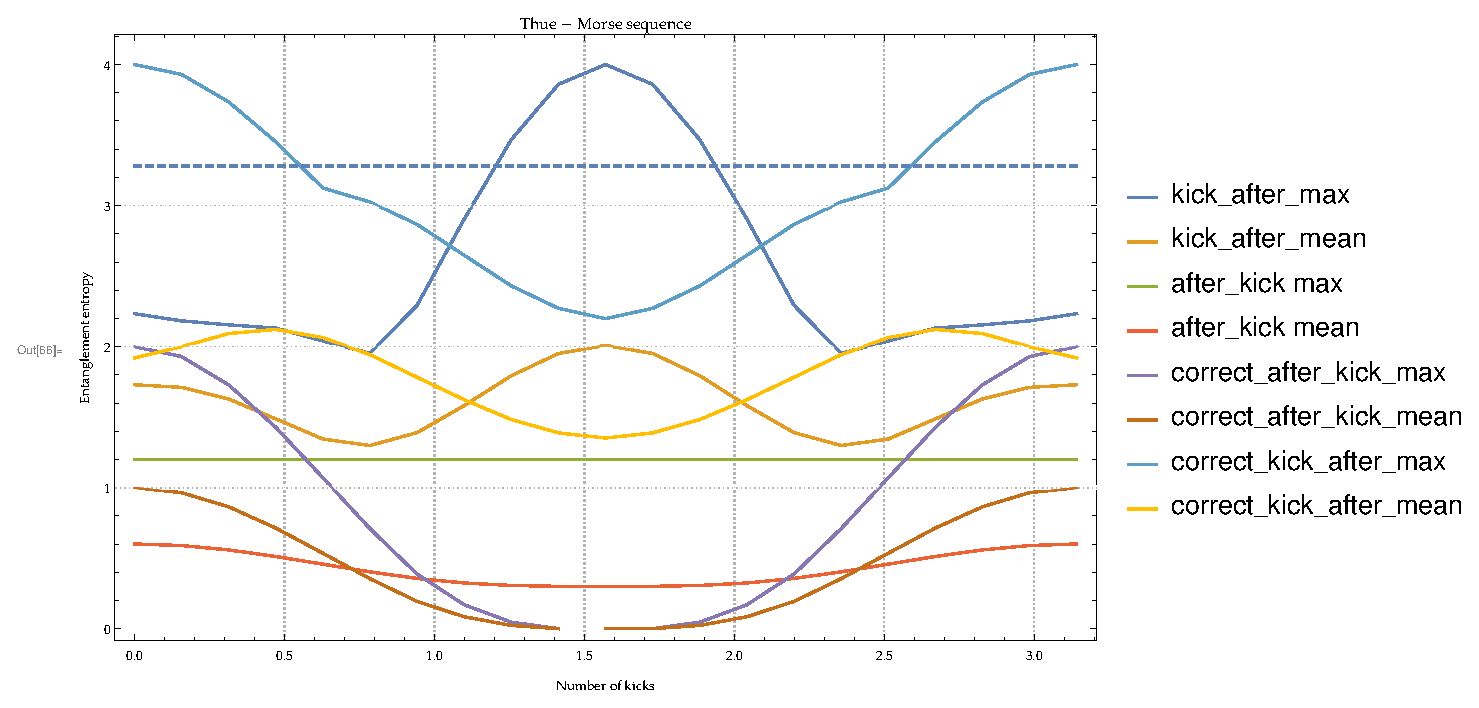
\includegraphics[scale=0.7,center]{thuemorsefinalall.eps}
 		\caption{The first four labels refer to the entanglement entropy in case of the tweaked Hamiltonian, while the next four labels refer to the initial kicked Ising Hamiltonian. "kick after" refers to the application of the Floquet operator in the order of Ukick Uafter  while "after kick" refers to the application of the Floquet operator Uafter Ukick}
		 \label{saturationwrong}
		  \end{figure}
		  
		
		  
		   \begin{figure}[h!]
     	  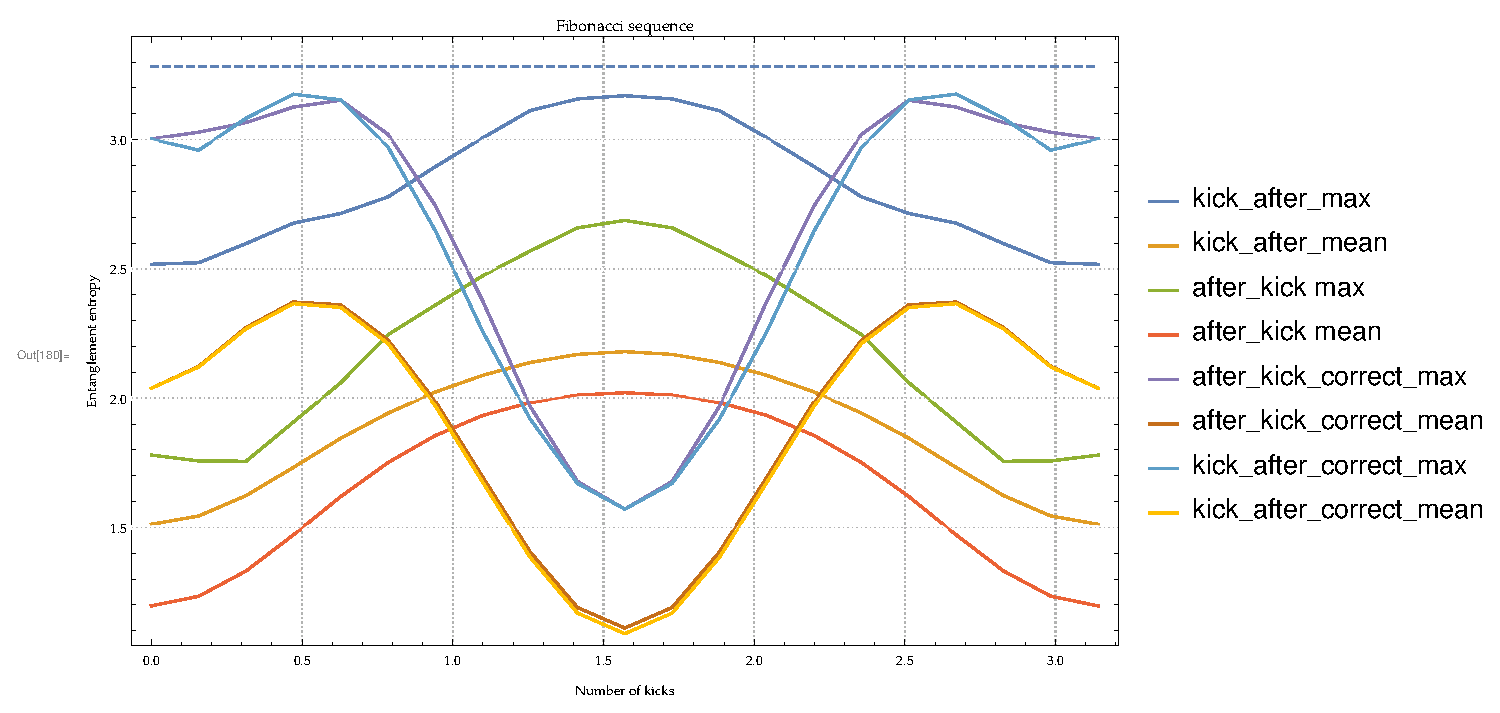
\includegraphics[scale=0.7,center]{fibofinalall.eps}
		 \caption{Fibonacci}
		 \label{saturationwrong}
		  \end{figure}
		   \begin{figure}[h!]
     	  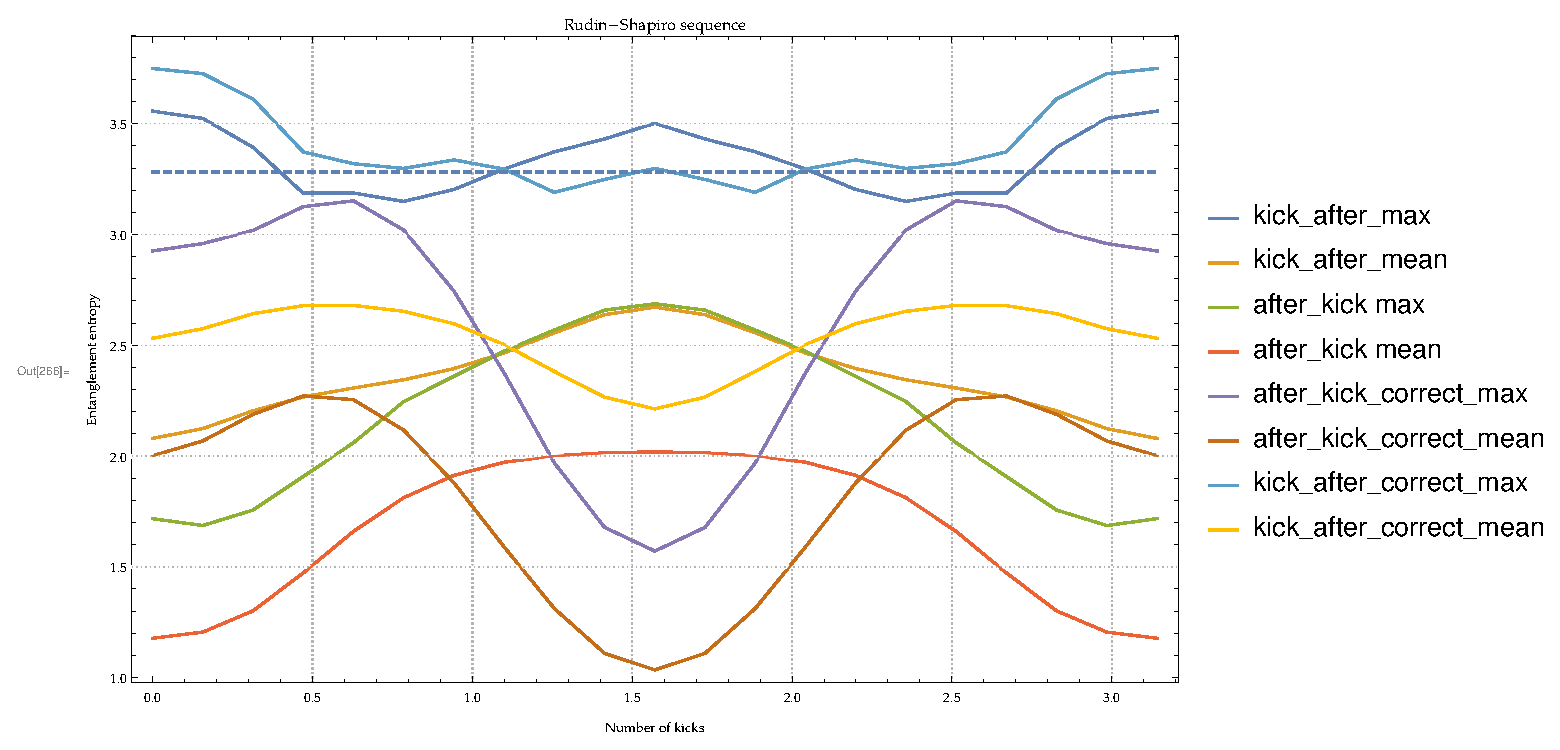
\includegraphics[scale=0.7,center]{rudinfinalall.eps}
		 \caption{Rudin Shapiro}
		 \label{saturationwrong}
		  \end{figure}
		  
		    \begin{figure}[h!]
     	  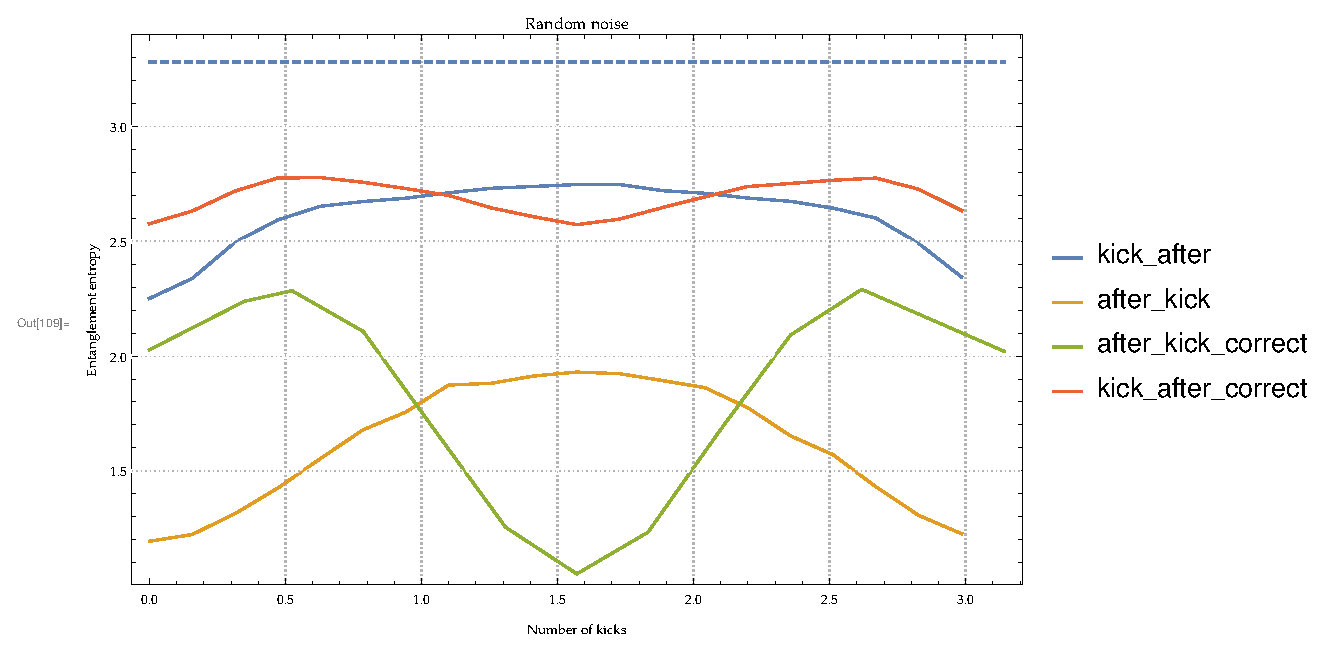
\includegraphics[scale=0.6,center]{noisefinaalll.eps}
		\caption{Random noise}
		 \label{saturationwrong}
		  \end{figure}
\end{figure}
\begin{comment}		  
	\subsection{Tweaking the Unitary operator}
	
		Suppose, interaction term and the magnetic field term are reversed in the time evolution operator making it look like: 
		
		\begin{equation}
		 U_{n} = \exp[-i
		 \dfrac{\pi}{4}(1+(\tau_{n+1}-\tau_{n})\dfrac{\text{dt}}{\pi/4})\sum_{j=1}^{L}\sigma_{j}^{z}]  \exp[-i\dfrac{\pi}{4}(1+\tau_{n}\dfrac{\text{dt}}{\pi/4})\sum_{j=1}^{L}\sigma_{j}^{x} \sigma_{j+1}^{x}]
		 \end{equation}
		 
		In the case when dt$=0$, the plots for entanglement entropy remains the same as before. But for dt $\neq 0$, we get different plots as shown in Figure     \ref{saturationwrong}

		
		
		  \begin{figure}[h]
		 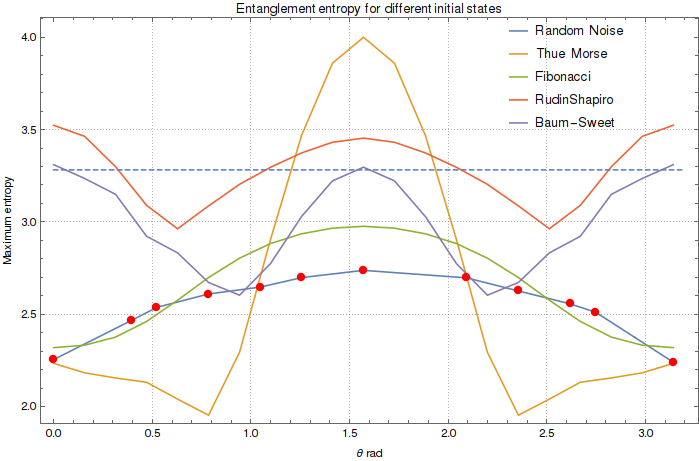
\includegraphics[scale=0.5,center]{sequences.png}
		 \caption{The dashed line is the average entropy of a totally random subsystem\cite{PhysRevLett.71.1291}. In the above figure Ising chain with 8 spins (periodic boundary conditions) is considered and entanglement is calculated between the two halves (4+4) spins. This is the case of tweaked Hamiltonian where the kick term came after the interaction term during unitary evolution }
		 \label{saturationwrong}
		  \end{figure}
		  
		  \end{comment}
		  
		  \subsection{Calculating Page entropy }
			Page entropy is the average entropy of a subsystem if the quantum system of the Hilbert space is in a pure random state. If the dimension of the Hilbert space is $mn$ the average entropy of the subsystem of dimension $m \leq n$ is given by $S_{m,n} = \sum_{k=n+1}^{mn} \dfrac{1}{k} - \dfrac{m-1}{2n}$. In this case, consider an 8-spin ising chain, so the dimension of the Hilbert space is $2^8$ and the subsystem with 4 spins will result in $m = 2^4$ and $n = 2^4$. So, 
			
			\begin{align}
			S_{16,16} &= \sum_{k = 17}^{256} \dfrac{1}{k} - \dfrac{15}{32}\\
			& = 2.274865969588287
\end{align}			 		  
		  But this value is taken with $\log_{e}$ but we have calculated the entanglement entropy with $\log_{2}$, so, diving the above obatined value with $\log_{e}2$ we get Page entropy to be:
		  
		  \begin{equation}
		  S_{16,16}  = \dfrac{2.274865969588287}{\log_{e}2} = 3.281937853012085
		  \end{equation}
		  
		 
        \subsection{Note on Jordan Wigner transformations}		 
		 
		
		
		
Let the Hamiltonian for 1D transverse field Ising chain be given in the following form:

\begin{equation}\label{spinh}
	H_{IM} = -J\sum_{n=1}^{N} \sigma^{z}_{n}\sigma^{z}_{n+1}  -h\sum_{n=1}^{N} \sigma^{x}_{n}
	\end{equation}

Consider the fermionic operator, $c_{j}$ at the $j^{th}$ site such that it satisfies the following commutation relations:

\begin{align}
\{c_{i},c_{j}^{\dagger}\} = \delta_{ij}\qquad
[c_{i},c_{j}] = 0
\end{align}
	
	Introducing the Majorana fermion operators with attached string operators such that the fermion antisymmetric properties under interchange between different sites is preserved is given by:
	
	\begin{align}
	\psi^{1}_{n} & = \dfrac{1}{\sqrt{2}}[ \prod_{l = 1}^{n-1}\sigma_{l}^{x}]\sigma_{n}^{y}\\
	\psi^{2}_{n} & = \dfrac{1}{\sqrt{2}}[ \prod_{l = 1}^{n-1}\sigma_{l}^{x}]\sigma_{n}^{z}
	\end{align} 
	
	Where $\psi^{1}_{j}$ and $\psi^{2}_{j}$ also satisfy :
	
	\begin{align}\label{m1}
	\psi^{1}_{j} &= \dfrac{c_{j}+c_{j}^{\dagger}}{2}\\
	\psi^{2}_{j} &= \dfrac{c_{j}^{\dagger}-c_{j}}{2i}
	\end{align}
	These Majorana fermions satistfy the relations:
	\begin{equation}
	\{ \psi_{i}^k,\psi_{j}^l \} = \delta_{ij}\delta_{kl}
	\end{equation}
	From the above equations, we can express the pauli matrices in terms of Majorana fermion operators:
	
	\begin{align}
	\sigma_{j}^{x} &= - 4i \psi^{1}_{j}\psi^{2}_{j}\\
	\sigma_{j}^{z}\sigma_{j+1}^{z} &=  4i \psi^{1}_{j}\psi^{2}_{j+1}
	\end{align}
	
	When periodic boundary conditions are imposed, the extra term in terms of Majorana fermions becomes $\sigma_{N}^z\sigma_{1}^z= -[\prod_{1}^N\sigma_{l}^x]2i\psi_{N}^1\psi_{1}^2 \equiv (-1)\cdot \mathcal{P}\cdot 2i\psi_{N}^1\psi_{1}^2 $ where $\mathcal{P} = [\prod_{1}^N\sigma_{l}^x]$ is the parity operator. 
	
	Consider the number operator given by $c_{j}^\dagger c_{j} = \dfrac{1+2i\psi_{j}^1\psi_{j}^2}{2} = \dfrac{1-\sigma_{n}^x}{2}$. 
	
	Writing $ \sigma^x =- i e^{1 \pi  \sigma^x/2} = e^{1\pi(\sigma^x-1) /2}  $, we can note that:
	
	\begin{equation}
	\mathcal{P} = \prod_{1}^N\sigma_{l}^x = (-1)^{\sum_{j=1}^N c_{j}^\dagger c_{j}}
	\end{equation}
	
	Now rewriting the Hamiltonian in terms of $\psi^{1}$ and $\psi^{2}$, we get :
	
		\begin{equation}
		H_{IM} = -\dfrac{J}{4i}\sum_{j=1}^{N} \psi_{j}^{1}\psi_{j+1}^{2} - \dfrac{h}{4i}\sum_{j=1}^{N} \psi_{j}^{1}\psi_{j}^{2}
		\end{equation}
		
		Substituting Eqns 28,29 we obtain the Hamiltonian in terms of $c_{j}$'s also, assuming periodic boundary conditions, we get:
		
		\begin{equation}
			H_{IM} = -J\sum_{j=1}^{N} (c_{j}^{\dagger}c_{j+1} + c_{j}^{\dagger}c_{j+1}^{\dagger}-c_{j}c_{j+1}-c_{j}c_{j+1}^{\dagger}) - 2h\sum_{j=1}^{N} c_{j}^{\dagger}c_{j}
		\end{equation}
	
     	Fourier transform of fermionic operators:
		\begin{equation}
		c_{j} = \dfrac{1}{\sqrt{N}}\sum_{k}d_{k} e^{i\pi kj/N}
		\end{equation}
		\begin{equation}
		d_{k} =  \dfrac{1}{\sqrt{N}}\sum_{j}c_{j} e^{-i\pi kj/N}
		\end{equation}
Note that, in the summation $k$ only takes odd/even values depending on antiperiodic/periodic boundary conditions. Here, since we are assming periodic boundary conditions, $k$ takes the following values:
\begin{align*}
k \epsilon \{\pm 1,\pm 3,...,\pm (N-1)\}
\end{align*}
	    
	    New hamiltonian in terms of $d_{k}$'s:
	    
	    \begin{equation}
	    		H_{IM} = -J\sum_{k\geq 0}^{ \pi (N-1)/N} (d_{k}^{\dagger}d_{k}e^{ik} + d_{k}^{\dagger}d_{-k}^{\dagger}e^{ik}-d_{k}d_{-k}e^{-ik}-d_{k}d_{k}^{\dagger}e^{-ik}) - 2h\sum_{k\geq 0}^{ \pi (N-1)/N} d_{k}^{\dagger}d_{k}
	    \end{equation}
	    
	    Simplified form:
	    
	    \begin{equation}
	    H_{IM} = -2\sum_{k\geq0}^{ \pi (N-1)/N}\begin{bmatrix}
	    d_{k}^{\dagger} & d_{-k}\\
	    \end{bmatrix} \begin{bmatrix}
	    h + J \cos(k) & i J \sin(k)\\
	    - i J \sin(k) & -h - J \cos(k) \\
	    \end{bmatrix}\begin{bmatrix}
	    d_{k}\\d_{-k}^{\dagger}\\
	    \end{bmatrix}
	    \end{equation}
	     
	    \subsubsection{Bogoliubov transformation}
	    The eigen values of $ M =  \begin{bmatrix}
	    h + J \cos(k) & i J \sin(k)\\
	    - i J \sin(k) & -h - J \cos(k) \\
	    \end{bmatrix}$ are $\pm |B_{k}|$ where:
	    \begin{equation}
	    |B_{k}| = \sqrt{J^{2}+h^{2}+2 J h \cos(k)}
	    \end{equation}
	    
	     \paragraph{   }
	    Let $b_{k} = J \sin(k) , c_{k} = h + J \cos(k)$
	    
	   
	    
	    	    The eigen vectors of M are $\dfrac{1}{Norm}\begin{bmatrix}
	    	    b_{k}\\i(c_{k}+\sqrt{b_{k}^{2}+c_{k}^{2}})\\
	    	    \end{bmatrix}  $ and $\dfrac{1}{Norm}\begin{bmatrix}
	    	    i(c_{k}+\sqrt{b_{k}^{2}+c_{k}^{2}})\\b_{k}\\
	    	    \end{bmatrix}  $ where $\dfrac{1}{Norm}$ is the normalization factor with 
	    	    \begin{equation}
	    	     Norm = \sqrt{2\sqrt{b_{k}^{2}+c_{k}^{2}}(c_{k}+\sqrt{b_{k}^{2}+c_{k}^{2}})}
	    	     \end{equation}
	    	   
	    	    \paragraph{   }
	    	    
	    	    Introducing a matrix 
	    	    \begin{equation}
	    	    U^{\dagger} = \dfrac{1}{Norm_{k}}\begin{bmatrix}
	    	    b_{k} & i(c_{k}+\sqrt{b_{k}^{2}+c_{k}^{2}})\\ i(c_{k}+\sqrt{b_{k}^{2}+c_{k}^{2}})& b_{k}\\
	    	    \end{bmatrix} 
	    	    \end{equation}
	    	    
	    	     and rewriting the Hamiltonian:
	    \begin{equation}
	      H_{IM} = -\sum_{k\geq 0}^{ \pi (N-1)/N}2\begin{bmatrix}
	      d_{k}^{\dagger} & d_{-k}\\
	      \end{bmatrix} U^{\dagger} \begin{bmatrix}
	     -|B_{k}| & 0\\
	      0 & |B_{k}| \\
	      \end{bmatrix}U\begin{bmatrix}
	      d_{k}\\d_{-k}^{\dagger}\\
	      \end{bmatrix}
	    \end{equation}
	    
	  Now let:
	    
	  
	    
	    	    
	     $ \begin{bmatrix}
	    d_{k}^{\dagger} & d_{-k}\\
	    \end{bmatrix} U^{\dagger} := \begin{bmatrix}
	    a_{k}^{\dagger} & a_{-k}\\
	    \end{bmatrix} $ and $ U\begin{bmatrix}
	    d_{k}\\d_{-k}^{\dagger}\\
	    \end{bmatrix}  := \begin{bmatrix}
	    a_{k}\\a_{-k}^{\dagger}\\
	    \end{bmatrix}$ we get:
	    
	    
		    \begin{equation}
		    H_{IM} = -2\sum_{k\geq 0}^{ \pi (N-1)/N}\begin{bmatrix}
		    a_{k}^{\dagger} & a_{-k}\\
		    \end{bmatrix}  \begin{bmatrix}
		   -|B_{k}| & 0\\
		    0 & |B_{k}| \\
		    \end{bmatrix}\begin{bmatrix}
		    a_{k}\\a_{-k}^{\dagger}\\
		    \end{bmatrix}
		    \end{equation}
		    
		    Simplifying the above equation we get:
		    
		    \begin{equation}
		     H_{IM} = 2\sum_{k\geq 0}^{ \pi (N-1)/N} (|B_{k}|a_{k}^{\dagger}a_{k}-|B_{k}|a_{-k}a_{-k}^{\dagger})
		    \end{equation}
		    
		    Considering the fact that $a_{k}$'s follow the same commutation relations as that of $d_{k}$'s the hamiltonian can be further simplified into:
		    
		    \begin{equation}
		    H_{IM} = 2\sum_{k=- \pi (N-1)/N}^{ \pi (N-1)/N} |B_{k}|(a_{k}^{\dagger}a_{k}-\dfrac{1}{2}) 
		    \end{equation}
		
	\subsubsection{Unitary operator after Jordan Wigner}
	
	Task: Express eqn 24 in terms of fermionic operators:
	\begin{align}
	H_{after} &= \sum_{i}\sigma_{i}^z \sigma_{i+1}^z
	\end{align}
	Here $J = -1$ and $h = 0$. So after the fourier tramsform of fermion operators the hamiltonian becomes:
	\begin{align}
	H_{after} = 2 \sum_{k \geq 0}^{\pi(N-1)/N} \begin{bmatrix}
	d_{k}^{\dagger} & d_{-k}
	\end{bmatrix} \begin{bmatrix}
	\cos k&i\sin k\\
	-i\sin k&-\cos k
	\end{bmatrix} \begin{bmatrix}
	d_{k}\\d_{-k}^{\dagger}
	\end{bmatrix}
	\end{align}
	
	Consider $M = \begin{bmatrix}
	\cos k&i\sin k\\
	-i\sin k&-\cos k
	\end{bmatrix}$, it has eigen values $\pm 1$ and eigen vectors $\begin{bmatrix}
	i\cos(k/2)\\ \sin(k/2)
	\end{bmatrix}$ and $\begin{bmatrix}
	\sin(k/2)\\i\cos(k/2)
	\end{bmatrix}$.\\\\
	
	Now consider the  matrix formed by the eigen vectors of $M$, $ U^\dagger = \begin{bmatrix}
	\sin(k/2)&i\cos(k/2)\\
	i\cos(k/2)&\sin(k/2)
	\end{bmatrix}$ such that $ U M U^\dagger  = \begin{bmatrix}
	-1&0\\0&1
	\end{bmatrix}$. This makes the hamiltonian:
	
     \begin{align}
     H_{after} &= 2\sum_{k \geq 0}^{\pi (N-1)/N}\begin{bmatrix}
     d_{k}^\dagger & d_{-k}
     \end{bmatrix}U^\dagger \begin{bmatrix}
     -1&0\\0&1
     \end{bmatrix}U \begin{bmatrix}
     d_{k}\\d_{-k}^\dagger
     \end{bmatrix}\\
     &=  2\sum_{k \geq 0}^{\pi (N-1)/N}\begin{bmatrix}
     d_{k}^\dagger & d_{-k}
     \end{bmatrix}\begin{bmatrix}
	\sin(k/2)&i\cos(k/2)\\
	i\cos(k/2)&\sin(k/2)
	\end{bmatrix} \begin{bmatrix}
     -1&0\\0&1
     \end{bmatrix}\begin{bmatrix}
	\sin(k/2)&-i\cos(k/2)\\
	-i\cos(k/2)&\sin(k/2)
	\end{bmatrix}\begin{bmatrix}
     d_{k}\\d_{-k}^\dagger
     \end{bmatrix}\\
\end{align}     	
	
	This gives the Bogoliubov transformed operators: 
	
	\begin{align}
	a_{k}^\dagger & = d_{k}^\dagger \sin(k/2) + id_{-k} \cos(k/2)\\
	a_{-k} &= id_{k}^\dagger \cos (k/2)+ d_{-k} \sin(k/2)\\
	a_{-k}^\dagger  &= -id_{k} \cos(k/2)+  d_{-k}^\dagger \sin(k/2)\\
	a_{k}&=d_{k} \sin(k/2) -i d_{-k}^\dagger \cos(k/2)
	\end{align}

So the Hamiltonian in the duration between consecutive kicks becomes:

\begin{align}
	H_{after} &= 2\sum_{k \geq 0}^{\pi (N-1)/N}\begin{bmatrix}
     a_{k}^\dagger & a_{-k}
     \end{bmatrix} \begin{bmatrix}
     -1&0\\0&1
     \end{bmatrix} \begin{bmatrix}
     a_{k}\\a_{-k}^\dagger
     \end{bmatrix}\\
	&=-2\sum_{k=- \pi (N-1)/N}^{ \pi (N-1)/N} (a_{k}^{\dagger}a_{k}-\dfrac{1}{2})  
	\end{align}	
	
	This makes the time evolution operator acting after a kick to be:
	
	\begin{equation}
	 U_{after} = \prod_{k>0} e^{i\dfrac{\pi}{4} a_{k}^\dagger a_{k}}e^{i\dfrac{\pi}{4} a_{-k}^\dagger a_{-k}} = \prod_{k=- \pi (N-1)/N}^{ \pi (N-1)/N} e^{i\dfrac{\pi}{4} a_{k}^\dagger a_{k}}
	 \end{equation} 
Note that the $\dfrac{1}{2}$ term in $(a_{k}^\dagger a_{k}- \dfrac{1}{2})$ can be ingnored as it merely adds  an overall phase to the unitary operator.

Now consider the second part of the overall Hamiltonian and call it $H_{kick}$. Note that this is \textbf{not} exactly the Hamiltonian at the time of the kick:

\begin{equation}
H_{kick} = \sum_{i}\sigma_{i}^x
\end{equation}

In this case $J = 0$ and $h = -1$. So after the Fourier transform of the fermion operators the Hamiltonian becomes:

\begin{equation}
H_{kick} = 2\sum_{k\geq0}^{ \pi (N-1)/N}\begin{bmatrix}
	    d_{k}^{\dagger} & d_{-k}\\
	    \end{bmatrix} \begin{bmatrix}
	    1 & 0\\
	    0 & -1 \\
	    \end{bmatrix}\begin{bmatrix}
	    d_{k}\\d_{-k}^{\dagger}\\
	    \end{bmatrix}
\end{equation}

The simplified Hamiltonian is:
	\begin{equation}
		H_{kick} = 2\sum_{k=- \pi (N-1)/N}^{ \pi (N-1)/N} (d_{k}^{\dagger}d_{k}-\dfrac{1}{2})  
		\end{equation}
	

The unitary operator that generates the time evolution at the instant of kick:
	\begin{equation}
	U_{kick} = \prod_{k>0} \exp(-i\dfrac{\pi}{4}\sum_{i}\sigma_{i}^x)
		\end{equation}
		
		This, after Jordan-Wigner transformation becomes:
		
	
		
		\begin{equation}
		U_{kick} = \prod_{k>0} e^{-i\dfrac{\pi}{4}d_{k}^\dagger d_{k}}e^{-i\dfrac{\pi}{4}d_{-k}^\dagger d_{-k}} = \prod_{k=- \pi (N-1)/N}^{ \pi (N-1)/N}e^{-i\dfrac{\pi}{4}d_{k}^\dagger d_{k}} 
		\end{equation}
		
		Where $d_{k}$'s  are the same Fourier transformed fermion  operators as defined before.
		The combined time-evolution is given by:
		\begin{align}
		U = U_{after}U_{kick} &= \prod_{k=- \pi (N-1)/N}^{ \pi (N-1)/N}e^{i\dfrac{\pi}{4} a_{k}^\dagger a_{k}}\prod_{l=- \pi (N-1)/N}^{ \pi (N-1)/N} e^{-i\dfrac{\pi}{4}d_{l}^\dagger d_{l}}\\
		&= \prod_{k=- \pi (N-1)/N}^{ \pi (N-1)/N}e^{i\dfrac{\pi}{4} a_{k}^\dagger a_{k}} e^{-i\dfrac{\pi}{4}d_{k}^\dagger d_{k}}
		\end{align} 
		
		A useful simplification:
		
		\begin{equation}
		e^{i\dfrac{\pi}{4}a_{k}^\dagger a_{k}} = 1 + a_{k}^\dagger a_{k}(e^{i\dfrac{\pi}{4}} -1) = 1 + a_{k}^\dagger a_{k}(\dfrac{1+i}{\sqrt{2}}-1)
		\end{equation}
		
		Implimenting this simplification and defining $U = \prod_{k=- \pi (N-1)/N}^{ \pi (N-1)/N} U_{k}$  we get:
		\begin{equation}
	U_{k} = 	(1 + a_{k}^\dagger a_{k}(\dfrac{1+i}{\sqrt{2}}-1))(1 + d_{k}^\dagger d_{k}(\dfrac{1-i}{\sqrt{2}}-1))
		\end{equation}
		
		Further simplification yeilds:
		
		\begin{align*}
		a_{k}^\dagger a_{k} &= (d_{k}^\dagger sin(k/2) + i d_{-k} \cos(k/2))(d_{k} \sin(k/2) -i d_{-k}^\dagger \cos(k/2)) \\
		&= d_{k}^\dagger d_{k}\sin^2(k/2) -i d_{k}^\dagger d_{-k}^\dagger cos(k/2)\sin(k/2) + d_{-k}d_{-k}^\dagger \cos^2(k/2) +i d_{-k}d_{k} \sin(k/2)\cos(k/2)
		\end{align*}
		
	%	$d_{-k}d_{-k}^\dagger = 1 - d_{-k}^\dagger d_{-k}$
		
	
		\begin{align*}
		a_{-k}^\dagger a_{-k} &= (-id_{k} \cos(k/2)+  d_{-k}^\dagger \sin(k/2))(id_{k}^\dagger \cos(k/2) + d_{-k}\sin(k/2))\\
		&= d_{k}d_{k}^\dagger \cos^2(k/2) -i d_{k}d_{-k}\sin(k/2)\cos(k/2) + id_{-k}^\dagger d_{k}^\dagger \sin(k/2)\cos(k/2) + d_{-k}^\dagger d_{-k} \sin^2(k/2)
		\end{align*}
		

		\begin{align*}
		a_{k}^\dagger a _{k} a_{-k}^\dagger a_{-k} &= -d_{k}^\dagger d _{k} d_{-k}^\dagger d_{-k} \sin^2(k/2)\cos k + d_{-k}d_{-k}^\dagger d_{k}d_{k}^\dagger \cos^2(k/2)\cos k-\\
		&\dfrac{i}{2}(d_{-k}^\dagger d_{k}^\dagger + d_{-k}d_{k})\sin(k)\cos(k) \\
		 d_{k}^\dagger d _{k} d_{-k}^\dagger d_{-k} &= (1-d_{k}d_{k}^\dagger)(1-d_{-k}d_{-k}^\dagger) = 1 + d_{k}d_{k}^\dagger d_{-k}d_{-k}^\dagger - (d_{k}d_{k}^\dagger + d_{-k}d_{-k}^\dagger)\\
a_{k}^\dagger a _{k} a_{-k}^\dagger a_{-k} &= 	d_{k}d_{k}^\dagger d_{-k}d_{-k}^\dagger \cos^2k	 
		\end{align*}
	
		
		\begin{align}\label{unitaryfinal}
		U &= 1 + (\dfrac{1+i}{\sqrt{2}}-1)((\cos k + 1 )(d_{k}^\dagger d_{k} + d_{-k}^\dagger d_{-k})+ \sin k(d_{k}d_{-k} + d_{-k}^\dagger d_{k}^\dagger )) \\&+ (\dfrac{1+i}{\sqrt{2}} -1)^2 (d_{-k}d_{k}^\dagger + 2 d_{k}^\dagger d_{k}d_{-k}^\dagger d_{-k}(\cos k +1 ))
		\end{align}
				
		Note that particle number is conserved upon the action of this unitary operator. Consider the all spin up state to be $||0\rangle \rangle$. In the fermionic language this refers to state in which all the fermions occupy the lower energy level such that $c|0\rangle = 0$ and $c^\dagger |0\rangle = |1\rangle$. So, this all spin up state will be the same thing in the fermionic basis. But it is different in the basis of $d_{k}$	operators. 
		
		The ground state is usually taken to be the all spin-up state. This state in the basis of $d_{k}$'s turns out to be the BCS ground state.
		
		\begin{equation}
		|\psi\rangle_{BCS} = \prod_{k>0}\dfrac{1}{ \sqrt{2(\cos k+1) }} (\sin k + i (\cos k +1 )d_{k}^\dagger d_{-k}^\dagger)||0\rangle \rangle
		\end{equation}
		
		Considering $\dfrac{\sin k}{\sqrt{2(\cos k + 1)}}  = \cos\theta_{k}$, and $\dfrac{\cos k + 1}{\sqrt{2(\cos k +1 )}} = \sin \theta_{k}$ we get : 
		
		\begin{equation}
		|\psi\rangle_{BCS} = \prod_{k>0} (\cos\theta_{k} + i \sin\theta_{k}d_{k}^\dagger d_{-k}^\dagger)||0\rangle\rangle
		\end{equation}
		 The time evolved state after n kicks looks like:
		 
		 \begin{equation}
		 |\psi(n)\rangle = U^n |\psi(0)\rangle
		 \end{equation}
		
%		What happens if I write the time-evolution operator in terms of Majorana fermions?
		
		Unitary operator for kicked Ising chain with noise incorporated:
		\begin{align}\label{noisyunitary}
	U_{n} = \prod_{k}U_{k} &= \prod_{k}	(1 + a_{k}^\dagger a_{k}(\dfrac{1+i}{\sqrt{2}}e^{i(\tau_{n+1}-\tau_{n})\text{dt}}-1))(1 + a_{-k}^\dagger a_{-k}(\dfrac{1+i}{\sqrt{2}}e^{i(\tau_{n+1}-\tau_{n})\text{dt}}-1))\\&*(1 + d_{k}^\dagger d_{k}(\dfrac{1-i}{\sqrt{2}}-1))(1 + d_{-k}^\dagger d_{-k}(\dfrac{1-i}{\sqrt{2}}-1))
		\end{align}
		So clearly this system is integrable. 

	This exercise was being performed for the interaction term $\sigma^z_{i}\sigma^z_{i+1}$, similarly, for the case in which interaction is along x and magnetic field along z, the Hamiltonian in fermion momentum space turns out to be:
	
	\begin{align}
			H_{kick} &= 2 \sum_{k}  [d_{k}^\dagger d_{k} - d_{-k}^\dagger d_{-k}]\\
			H_{after} &= -2\sum_{k}(  \cos k [d_{k}^\dagger d_{k} - d_{-k}^\dagger d_{-k}] -  \sin k [d_{-k}d_{k} + d_{k}^\dagger d_{-k}^\dagger])
			\end{align}		
			
			Now let us define a new space whose basis states are $ |0\rangle $ (which is the no fermion state in the momentum basis) and $ d_{k}^\dagger d_{-k}^\dagger |0\rangle $. Hamiltonian takes this simple form in this basis:
			
			\begin{align}
			H_{kick} &= -2 \sum_{k}  \sigma_{k}^z\\
			H_{after} &= 2\sum_{k} (\cos k \sigma_{k}^z - \sin k \sigma_{k}^x )
			\end{align}	
			
			
	The initial state is taken to be the ground state of the interaction Hamiltonian. In this newly defined basis, it takes the following form:
		
		\begin{equation}\label{key}
		 |\psi(0)\rangle_{k} = v_{k}(0) |0\rangle + u_{k}(0) |1\rangle
		\end{equation}
		
		Where $ v_{k}(0) = \sin(k/2) $ and $ u_{k}(0) = \cos(k/2) $
		
		Now the unitary evolution of this initial state is: 
		
		\begin{equation}\label{key}
		i \dfrac{d}{dt} \begin{bmatrix}
		v_{k}(t)\\u_{k}(t)
		\end{bmatrix} =  H_{k}\begin{bmatrix}
			v_{k}(t)\\u_{k}(t)
		\end{bmatrix}
		\end{equation}
		
		Now since $ H_{k} $ is in the form of  2 x 2  matrices, the numerical computation of the evolution of the states becomes exponentially faster. 
 		
 		Lets us see what the Floquet operator looks like in this case, for the particular case where the time period is $ \dfrac{\pi}{4} $: 
 		
 			\begin{align}
 		U_{kick}& = \exp(-i \dfrac{\pi}{4} H_{kick})\\
 		& = \exp(i \dfrac{\pi}{2} \sum_{k}\sigma_{k}^z)\\
 		& = i\prod_{\otimes k} \sigma_{k}^z\\
 		U_{after} & = \exp(-i\dfrac{\pi}{4}H_{after})\\
 		&= \exp(-i\dfrac{\pi}{2}\sum_{k} (\cos k \sigma_{k}^z - \sin k \sigma_{k}^x ))\\
 		& = -i \prod_{\otimes k} (\cos k \sigma_{k}^z - \sin k \sigma_{k}^x )
 		\end{align}
 		
 	In the presence of no noise, the Floquet operator takes the simple form: 
 	
 	\begin{equation}\label{key}
 	U = - \prod_{\otimes k} (\cos k - \sin k \sigma_{k}^x \sigma_{k}^z)
  	\end{equation}
  	
  	Note that this simple expression for the Floquet operator occurs only for the case when the period of the kicks happens to be $ \pi/4 $ which is a special case where the system sees symmetries. 
  	
  	
  	In the presence of noise, the unitary operator for the kth mode  turns out to be (with $ \epsilon $ being 0 or 1 with a probability of 1/2 ) and $ U_{j} $  the unitary operator acting after $ j $ periods\cite{PhysRevB.98.064305}: 
  	
  	\begin{align}
  	U_{kick} &= (i\sigma_{k}^z)^\epsilon\\
  	U_{after}& =  -i  (\cos k \sigma_{k}^z - \sin k \sigma_{k}^x )
  	\end{align}
  	
  	\begin{align}
  	U_{j} &=   \begin{bmatrix}
  	\cos k & -\sin k\\
  	-\sin k & -\cos k \\ 
  	\end{bmatrix} \begin{bmatrix}
  	1& 0 \\
  	0 & (-1)^{\epsilon_{j}}\\
  	\end{bmatrix} =  \begin{bmatrix}
  	\cos k & -(-1)^{\epsilon_{j}}\sin k \\
  	-\sin k & -(-1)^{\epsilon_{j}}\cos k \\  
  	\end{bmatrix}\\
   	U_{j}U_{l} 	&=  \begin{bmatrix}
  	\cos k & -(-1)^{\epsilon_{j}}\sin k \\
  	-\sin k & -(-1)^{\epsilon_{j}}\cos k \\  
  	\end{bmatrix}  \begin{bmatrix}
  	\cos k & -(-1)^{\epsilon_{l}}\sin k \\
  	-\sin k & -(-1)^{\epsilon_{l}}\cos k \\  
  	\end{bmatrix}\\
  	& = \begin{bmatrix}
  	\cos^2 k + (-1)^{\epsilon_{j}}\sin^2 k & \cos k \sin k(-(-1)^{\epsilon_{j}} + (-1)^{\epsilon_{j}+\epsilon_{l}})\\
  	\sin k \cos k (-1 + (-1)^{\epsilon_{j}})& (-1)^{\epsilon_{l}}\sin^2 k + (-1)^{\epsilon_{j}+\epsilon_{l}}\cos^2  k\\
  	\end{bmatrix}
    	\end{align}
 	
 	
 	
 	
 	
 	
		\subsection[Geometric picture]{Visualizing k-mode evolution on the Bloch sphere}
		
		Now that we have $ \begin{bmatrix}
		v_{k}(t)\\u_{k}(t)
		\end{bmatrix} $ for any t, we would want to visualize this time evolution on the Bloch sphere. 
		
		Consider a single k-mode:
		
		\begin{align}
		\begin{bmatrix}
		v_{k}(t)\\u_{k}(t)
		\end{bmatrix}  & = e^{i\beta} \cos[\dfrac{\theta}{2}] |0\rangle + e^{i\alpha} \sin[\dfrac{\theta}{2}] |1\rangle \\
		&=   e^{i\beta}(\cos[\dfrac{\theta}{2}] |0\rangle + e^{i(\alpha-\beta)} \sin[\dfrac{\theta}{2}] |1\rangle)
		\end{align}
		
		
		
		
		Now we need to find out $ \theta  $ and $ (\alpha-\beta) $. This can be found out from the following constraints. 
		
		\begin{align}
		|v_{k}|^2 + |u_{k}|^2 &= 1  \\ 
		\theta & = 2 \cos^{-1} (|v_k|)	\\
		e^{i\beta} = v_k/\cos(\theta/2)	\\
		e^{i(\alpha-\beta)} = \dfrac{u_k}{v_k} \cot(\theta/2)
				\end{align}
				
				
		With the parameters $ \theta  \text{and} (\alpha - \beta) $ know, we can now plot the k-mode evolution on the Bloch sphere. Notice that in this special case where the time period is taken to be $ \pi/4 $ the action of the Floquet operator does not bring about any change to the relative phase i.e., $ (\alpha- \beta) $. We start off with the initial state whose parameters $ \theta_{0}$ and $\phi_{0} = (\alpha_{0} - \beta_{0}) $ are known. 
		
		\begin{figure}
			\centering
			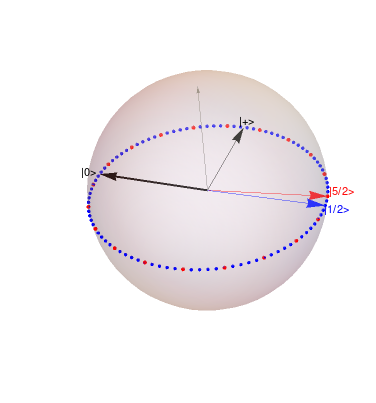
\includegraphics[width=0.7\linewidth]{piby4blochsphere}
			\caption{k-mode evolution, when  $T = \pi/4 $. The colored arrow shows the initial states for two modes $ k  = \pi/100 $ and $ k = 5\pi/100 $ }
			\label{fig:piby4blochsphere}
		\end{figure}
	
	\begin{figure}
		\centering
		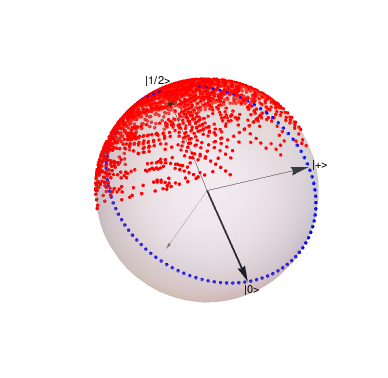
\includegraphics[width=0.5\linewidth]{blochsphere_half_01}
		\caption{k-mode evolution, when  $T = \pi/4 + 0.01 $ shown  in red for  $ k  = \pi/100 $ and the blue points correspond to $ T = \pi/4 $}
		\label{fig:blochspherehalf01}
	\end{figure}
	\begin{figure}
		\centering
		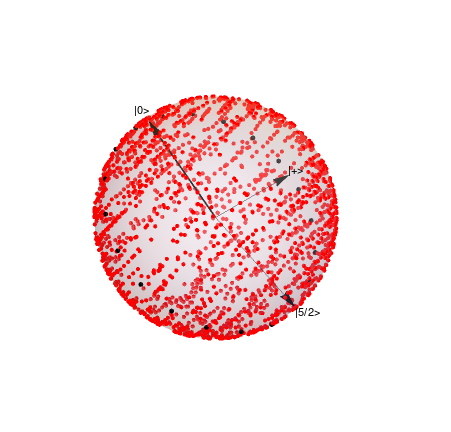
\includegraphics[width=0.5\linewidth]{blochsphere_fiveby2_01}
		\caption{k-mode evolution, when  $T = \pi/4 + 0.01 $ shown  in red for  $ k  = 5\pi/100 $ and the blue points correspond to $ T = \pi/4 $}
		\label{fig:blochspherefiveby201}
	\end{figure}
	
	
		
		
		\subsection{Entanglement Entropy of the fermion subsystem}
		Finding the entanglement entropy of the subsystem from the reduced density matrix\cite{Peschel_2009}. The reduced density matrix for this fermionic system can be obtained in the following manner\cite{Peschel_2003} by calculating the correlation matrix    \cite{Latorre_2009} and relating it to the reduced density matrix of the block. 
		
\subsubsection{Calculating Reduced density matrix from correlation functions}		

Any density matrix can be expressed as:

\begin{equation}\label{rho_exp}
\rho = \dfrac{1}{\mathcal{Z}}\exp(-\beta \mathcal{H})
\end{equation}

Where $ \mathcal{H} $ is a Hermitian matrix, $ \beta $ is a constant and $ \mathcal{Z} $ is the normalization factor (partition function). This way of expression can be justified by noting that $ \rho $ is always positive definite and $ Tr[\rho] = 1 $, and Eq.\eqref{rho_exp} satisfies both these conditions. 

Any general Hermititan operator for a system comprising of N 2-state particles can be written in terms of Pauli matrices and Identity operator as:

\begin{equation}\label{key}
\mathcal{H} = \prod_{\otimes k}(\vec{B_{k}}\cdot\vec{\sigma}+\mu_{k}\mathcal{I})
\end{equation} 

In the case of free fermions hopping between lattices the Hamiltonian has the form: 

\begin{equation}\label{key}
\hat{H}  = - \sum_{n,m} \hat{t}_{nm}c_{n}^\dagger c_{m}
\end{equation}

The reduced density matrix of a subsystem with $ M $ sites formed by the combination of eigenvectors of the above Hamiltonian can be expressed in the following form:

\begin{equation}\label{key}
\rho  = \dfrac{1}{\mathcal{Z}} \exp(-\sum_{i,j}H_{ij}c_{i}^\dagger c_{j})
\end{equation}

Let us denote $ \mathcal{H} = -\sum_{i,j}H_{ij}c_{i}^\dagger c_{j}  $. 

Diagonalizing $ \mathcal{H} $ by exploiting its eigenvectors $ \phi_{k} $ and eigenvalues $ \epsilon_{k} $   such that 

\begin{equation}\label{key}
c_{i} = \sum_{k} \phi_{k}(i) a_{k}
\end{equation}

Now $ \rho $ becomes 

\begin{equation}\label{kedy}
\rho  = \dfrac{1}{\mathcal{Z}} \exp(-\sum_{k = 1}^{M}\epsilon_{k}a_{k}^\dagger a_{k})
\end{equation}

Now consider the correlation matrix given by:

\begin{equation}
\hat{C}_{mn} = \langle c_{m}^\dagger c_{n}\rangle
\end{equation}



By exploiting the properties of free fermion system, we can note that:

\begin{equation}
\langle c_{n}^\dagger c_{m}^\dagger c_{k}c_{l}\rangle = \langle c_{n}^\dagger c_{l}\rangle \langle c_{m}^\dagger c_{k}\rangle-\langle c_{n}^\dagger c_{k}\rangle \langle c_{m}^\dagger c_{l}\rangle
\end{equation}

We know that:
\begin{equation}
\langle c_{m}^\dagger c_{n}\rangle = Tr[\rho c_{m}^\dagger c_{n}]
\end{equation}

Now the problem is to find the reduced density matrix using the correlation functions. From Wick's theorem, $\rho$ can be decribed in terms of fermions as follows:

\begin{equation}
\rho = K e^{-\sum_{i,j}H_{ij}c_{i}^\dagger c_{j}}
\end{equation}

Diagonalizng the $H$ matrix with its eigen values being $\epsilon_{k}$ with eigen functions being $ \phi_{k} (i)$. The diagonalizaiton process is done in the following way:

\begin{equation}
c_{i} = \sum_{k}\phi_{k}(i)a_{k}
\end{equation}

With this the density matrix now becomes:

\begin{equation}
\rho = K e^{-\sum_{k}\epsilon_{k}a_{k}^\dagger a_{k}}
\end{equation}

Finally the eigen values $\chi_{k}$ of $\hat{C}$ and $\epsilon_{k}$ of $H$ are related by:

\begin{equation}
\chi_{k}  =(e^{\epsilon_{k}} +1)^{-1}
\end{equation}

In matrix form:

\begin{equation}
H^T = \ln [(1-C)/C]
\end{equation}
		
		Therefore $\rho $ can be comlpetely determined once $\hat{C}$ is known. 
	
Now consider the case of kicked Ising chain. Correlation matrix in this case after Fourier transforming the fermion operators is given by: 
		
		\begin{align}
		D_{kl} &= \langle d_{k}^\dagger d_{l} \rangle =\dfrac{1}{N} \langle \sum_{m} e^{ikm} c_{m}^\dagger\sum_{n} e^{-iln}c_{n}\rangle \\
		D_{kl} &= \dfrac{1}{N}\sum_{m,n} e^{i\pi(mk-nl)/N}C_{mn}\\
		C_{mn}&=  \dfrac{1}{N}\sum_{k,l} e^{-i\pi(mk-nl)/N}D_{kl}
		\end{align}
		
		Given that the unitary operator is given by \ref{noisyunitary} the state is evolved in the $d_{k}$ basis. The correlation matrix $\hat{C}$ can be calculated by taking the Fourier transform of the correlation matrix in $d_{k}$ basis. 
Let the initial state be defined to be $|\psi(0)\rangle$ the state after N kicks is given by $U^N |\psi(0)\rangle$. The correlation matrix after N kicks happens to be :

\begin{align}
D_{mn}(N) &= \dfrac{1}{N} \langle \psi(0)|U^{\dagger N} d_{m}^\dagger d_{n}  U^{ N}| \psi(0)\rangle\\
C_{mn}(N) &= \dfrac{1}{N} \sum_{k,l} e^{-i\pi(mk-nl)/N} \langle \psi(0)|U^{\dagger N} d_{k}^\dagger d_{l}  U^{ N}| \psi(0)\rangle
\end{align}		


Another correlation matrix, $ F $ is defined as:

\begin{equation}\label{key}
F_{mn}(N) = \dfrac{1}{N} \sum_{k,l} e^{-i\pi(mk+nl)/N} \langle \psi(0)|U^{\dagger N} d_{k}^\dagger d_{l}^\dagger  U^{ N}| \psi(0)\rangle
\end{equation}

Taking into account both these correlation matrices, the $ 2l \times 2l $ matrix $ \mathcal{C}[2l] $ is formed:

\begin{equation}\label{key}
\mathcal{C} = \begin{bmatrix}
I - C & F\\
F^\dagger & C\\
\end{bmatrix}
\end{equation}

So this was done for the reduced density matrix in the fermion space. How can we correlate to the reduced density matrix in the spin space? 


 
\textbf{Claim} : Von Neumann entropy of the eigen values of $ \mathcal{C}  $ is the same as the Von Neumann entropy of the reduced density matrix of the subsystem of length $ l $. With this, the correlation matrix can be easily calculated and we can obtain the entanglement entropy.


\begin{figure}
	\centering
	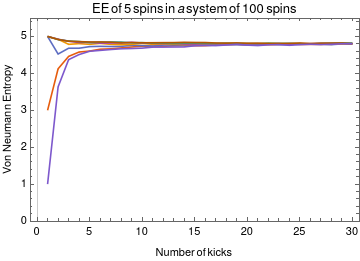
\includegraphics[width=0.7\linewidth]{5_95_EE}
	\caption{}
	\label{fig:595ee}
\end{figure}
\begin{figure}
	\centering
	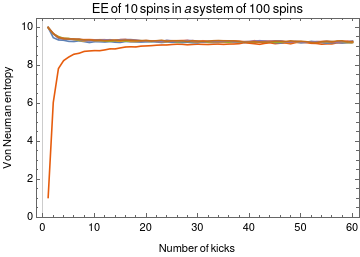
\includegraphics[width=0.7\linewidth]{10_90_EE}
	\caption{}
	\label{fig:1090ee}
\end{figure}

\begin{section}{Remarks}
	\begin{itemize}
		\item Eigen value spectra of the reduced density matrix needs to be calculated in order to look for signs of quantum chaos and thermalization
		\item Aperiodicity along the lines of Thue Morse, Fibonacci sequences also shows interesting entanglement behaviour. 
	\end{itemize}
\end{section}

\begin{comment}
Next we find out the distribution of eigen values of the reduced density matrix from the information obtained from the correlation matrices. 

Question: How can the eigen values of the reduced density matrix be found out from the eigen values of $ \mathcal{C} $ ?  
\end{comment}

		
		
%		\newpage
		
		
		
		
		
		
		
		
		
		
		
		
		
	\begin{comment}	
	
	Calculating the entanglement entropy 
		
		\section{Aperiodically Driven Integrable Systems and Their Emergent Steady States}
		
		

			Transverse field Ising Hamiltonian (periodic boundary condition): 
			\begin{equation}
			H_{IM} = -\sum_{n=1}^{N} \sigma^{z}_{n}\sigma^{z}_{n+1}  -g(t)\sum_{n=1}^{N} \sigma^{x}_{n}
			\end{equation}
			where g(t) is the strength of the external magnetic field which happens to be time dependent.
			\subsection{Fermionic description}
			By performing Jordan-Wigner transformations as described in sec 2.2, rewriting the Hamiltonian in terms of Majorana fermions $\psi^{1}$ and $\psi^{2}$, we get :
			
			\begin{equation}
			H_{IM} = -\dfrac{1}{4i}\sum_{j=1}^{N} \psi_{j}^{1}\psi_{j+1}^{2} - \dfrac{g(t)}{4i}\sum_{j=1}^{N} \psi_{j}^{1}\psi_{j}^{2}
			\end{equation}
			
		 The Hamiltonian in terms of $c_{j}$'s
			
			\begin{equation}
			H_{IM} = -\sum_{j=1}^{N} (c_{j}^{\dagger}c_{j+1} + c_{j}^{\dagger}c_{j+1}^{\dagger}-c_{j}c_{j+1}-c_{j}c_{j+1}^{\dagger}) - 2g(t)\sum_{j=1}^{N} c_{j}^{\dagger}c_{j}
			\end{equation}
			
			Fourier transform of fermionic operators:
			\begin{equation}
			c_{j} = \dfrac{1}{\sqrt{N}}\sum_{k = -\pi N/N}^{ \pi (N-1)/N}d_{k} e^{ikj}
			\end{equation}
			\begin{equation}
			d_{k} =  \dfrac{1}{\sqrt{N}}\sum_{j = -\pi N/N}^{ \pi (N-1)/N}c_{j} e^{-ikj}
			\end{equation}
			
			
			New hamiltonian in terms of $d_{k}$'s:
			
			\begin{equation}
			H_{IM} = -\sum_{k=0}^{ \pi (N-1)/N} (d_{k}^{\dagger}d_{k}e^{ik} + d_{k}^{\dagger}d_{-k}^{\dagger}e^{ik}-d_{k}d_{-k}e^{-ik}-d_{k}d_{k}^{\dagger}e^{-ik}) - 2g(t)\sum_{k=0}^{2 \pi (N-1)/2} d_{k}^{\dagger}d_{k}
			\end{equation}
			
			Simplified form:
			
			\begin{equation}
			H_{IM} = -2\sum_{k=0}^{ \pi (N-1)/2}\begin{bmatrix}
			d_{k}^{\dagger} & d_{-k}\\
			\end{bmatrix} \begin{bmatrix}
			g(t) +  \cos(k) & i  \sin(k)\\
			- i  \sin(k) & -g(t) -  \cos(k) \\
			\end{bmatrix}\begin{bmatrix}
			d_{k}\\d_{-k}^{\dagger}\\
			\end{bmatrix}
			\end{equation}
	
		The hamiltonian for each mode is given by:
		
		\begin{align}
		H_{k} & = \begin{bmatrix}
		d_{k}^{\dagger} & d_{-k}\\
		\end{bmatrix} \begin{bmatrix}
		g(t) +  \cos(k) & i  \sin(k)\\
		- i  \sin(k) & -g(t) -  \cos(k) \\
		\end{bmatrix}\begin{bmatrix}
		d_{k}\\d_{-k}^{\dagger}\\
		\end{bmatrix}\\
		& = (g(t)+\cos(k))(d_{k}^{\dagger}d_{k}-d_{-k}d_{-k}^{\dagger})+i \sin(k)(d_{k}^{\dagger}d_{-k}^{\dagger}-d_{-k}d_{k})
		\end{align}


\subsection{Driving Protocol}

	The system is driven with some pertubations added into it in terms of noise. This driving protocol is given as follows:
	
	\begin{equation}
	U_{k}(T)  = exp(-iH_{k}(g_{f}\dfrac{T}{2}))exp(-iH_{k}(g_{i}\dfrac{T}{2}))
	\end{equation}
	
	The perturbed Floquet dynamics can be given by : 
	
	\begin{equation}
	|\phi_{k}(n)\rangle = \mathcal{T}\prod_{i=1}^{n}U_{k}(T+\tau_{i}dT)
	\end{equation}
	\subsection{Representing the modes on the Bloch sphere}
	
		Consider the vector $\vec{B_{k}} = (0,J\sin(k),h+J\cos(k))$ and $ \vec{\sigma}=(\sigma^{x},\sigma^{y},\sigma^{z})$. $\vec{B_{k}}\cdot\vec{\sigma} = M$ where M is the matrix of the Hamiltonian when expressed in terms of fermion operators in momentum space. 
		\\
		\\
		Let $\vec{B_{k}}$ represent a magnetic field vector. The ground state vector associated with this magnetic field is the eigen state of M with the eigenvalue $-\sqrt{h^{2}+J^{2}+2hJ\cos(k)}$. The eigen state is 
		\begin{equation}
		|\phi\rangle =  \dfrac{1}{_{Norm_{k}}}\begin{bmatrix}
		Jsin(k)\\i(h+J\cos(k)+\sqrt{h^{2}+J^{2}+2hJ\cos(k)})\\
		\end{bmatrix} = \begin{bmatrix}
		\cos(\theta)\\i\sin(\theta)
		\end{bmatrix}
		\end{equation}
		
		
		\begin{align*}
		|\phi\rangle &= \begin{bmatrix}
		\cos(\theta)\\i\sin(\theta)
		\end{bmatrix} =  \cos\dfrac{\alpha}{2}\begin{bmatrix}
		1\\0
		\end{bmatrix} + e^{i\pi/2}\sin\dfrac{\alpha}{2} \begin{bmatrix}
		0\\1
		\end{bmatrix} 
		\end{align*}
		
	  where $\theta = \alpha/2$
		 Let $\begin{bmatrix}
		 1\\0
		 \end{bmatrix} := |0\rangle $ and $\begin{bmatrix}
		 0\\1
		 \end{bmatrix} := |1\rangle $\\
		  which gives $	|\phi\rangle =  \cos\dfrac{\alpha}{2} |0\rangle  + e^{i\pi/2}\sin\dfrac{\alpha}{2}  |1\rangle $
		 
		Acting the time evolution operator according to the driving protocol we get:
		 
		 \begin{align*}
		 |\phi(t)\rangle& = e^{it\gamma\vec{B_{k}}'\cdot\vec{\sigma}}|\phi(0)\rangle\\
		 &= e^{it\gamma\vec{B_{k}}'\cdot\vec{\sigma}}(\cos\dfrac{\alpha}{2} |0\rangle  + e^{i\pi/2}\sin\dfrac{\alpha}{2}  |1\rangle )\\
		 \vec{B_{k}}'\cdot\vec{\sigma} & = J'\sin k\sigma^{y}+ (h'+J'\cos k)\sigma^{z}\\
		 \vec{B_{k}}'\cdot\vec{\sigma}\:|0\rangle & = -iJ'\sin k|1\rangle+ (h'+J'\cos k)|0\rangle\\
		 \vec{B_{k}}'\cdot\vec{\sigma}\:|1\rangle & = iJ'\sin k|0\rangle- (h'+J'\cos k)|1\rangle\\
		 e^{it\gamma\vec{B_{k}}'\cdot\vec{\sigma}}&= 1 \cos(\gamma t |B'_{k}|) + i\dfrac{ \vec{B_{k}'\cdot\vec{\sigma}}}{|B'_{k}|}\sin(\gamma t |B'_{k}|)
		 \end{align*}
		 
		 
		 \subsection{Reduced density matrices and distance measure}
		 Consider a Hamiltonian $\hat{H}=$
		 \begin{align}
		 \langle c_{n}^\dagger c_{m}^\dagger c_{k} c_{l}\rangle &=  ?\\
		  c_{m}^\dagger c_{k} &= \delta_{mk} - c_{k} c_{m}^\dagger\\
		  c_{n}^\dagger c_{m}^\dagger c_{k} c_{l} & = c_{n}^\dagger(\delta_{mk} - c_{k} c_{m}^\dagger)c_{l}\\
		  & = c_{n}^\dagger\delta_{mk}c_{l} - c_{n}^\dagger c_{k} c_{m}^\dagger c_{l}\\
		  & = c_{n}^\dagger c_{l}\delta_{mk} -c_{n}^\dagger c_{k} (\delta_{ml} - c_{l}c_{m}^\dagger)\\
		  &= 
		 \end{align}
		 
	\subsection{Coarse Graining method}
	wvwwv
		 
		
		 
		\subsection{Plots}
		
	 		 
		 
		 \subsection{codes}
		 
	

		
		 

		 
	
\end{comment}

\begin{comment}
\section{Ising model with tilted magnetic field}
	Defining the Hamiltonian:
	    \begin{equation}
	        H = J\sum_{i=0}^{N}\sigma_{i}^{z}\sigma_{i+1}^{z}+h_{z}\sum_{i=0}^{N}\sigma_{i}^{z}+h_{x}\sum_{i=0}^{N}\sigma_{i}^{x}
	     \end{equation}
	    Let,
	    
	    \begin{align}
	    H_{1} &= J\sum_{i=0}^{N}\sigma_{i}^{z}\sigma_{i+1}^{z}+h_{z}\sum_{i=0}^{N}\sigma_{i}^{z}\\
	    H_{2}&=h_{x}\sum_{i=0}^{N}\sigma_{i}^{x}
	    \end{align} 
	    
	    Time evolution operator looks like $ e^{iHt} =e^{i(H_{1}+H_{2})t}  $. In the limit $ \Delta t \rightarrow 0 $ , $ e^{i(H_{1}+H_{2})\Delta t} = e^{iH_{1}\Delta t}e^{iH_{2}\Delta t}   $
	    
	    \begin{equation}
	    e^{iH\Delta t}|\psi\rangle = e^{iH_{2}\Delta t}e^{iH_{1}\Delta t}|\psi\rangle
	    \end{equation}
	
	Now $ |\psi\rangle $ is expressed in the eigen basis of $ \sigma^{z} $ so, $ e^{iH_{1}\Delta t}|\psi\rangle = |\psi\rangle e^{iE_{1}\Delta t}$ where, $ E_{1} $ is the eigenvalue. 
	\subsection{Fast Walsh-Hadamard Transformation}
	
		Consider the Hadamard operator $ \mathbb{H} =\dfrac{1}{\sqrt{2}} \begin{bmatrix}
	     1&1\\
	     1&-1\\
		\end{bmatrix} $. Note that $ \mathbb{H} \sigma^{z}\mathbb{H} =  \sigma^{x} $. Now applying this in Eq(3) we get:,  
		\begin{align}
			H_{2} &=  h_{x}\sum_{i=0}^{N}\mathbb{H}_{N}\sigma_{i}^{z}\mathbb{H}_{N}\qquad \text{where},\qquad \mathbb{H}_{N} = \otimes_{N}\mathbb{H} \\
			 e^{iH_{2}\Delta t}e^{iH_{1}\Delta t}|\psi\rangle&=  e^{iH_{2}\Delta t}e^{iH_{1}\Delta t}|\psi\rangle
		\end{align}
		
		Since $ H_{1} $ is already a diagonal matrix,  $ e^{iH_{1}\Delta t}|\psi\rangle = |\psi_{1}\rangle $ can be easily computed. Now coming to $ e^{iH_{2}\Delta t}|\psi_{1}\rangle  $\footnote{Note that $ \mathbb{H}^{2} = \begin{bmatrix}
			1&0\\
			0&1\\ 
			\end{bmatrix} = I$ and $ \sigma^{x2}= I $}, 
		\begin{align}
		e^{iH_{2}\Delta t}|\psi_{1}\rangle &= e^{ih_{x}\sum_{i=0}^{N}\mathbb{H}_{N}\sigma_{i}^{z}\mathbb{H}_{N}\Delta t}|\psi_{1}\rangle\\
		&=e^{ih_{x}\mathbb{H}_{N}(\sum_{i=0}^{N}\sigma_{i}^{z})\mathbb{H}_{N}\Delta t}|\psi_{1}\rangle\\
		& = \cos(h_{x}\Delta t)I_{N}|\psi_{1}\rangle + i \sin(h_{x}\Delta t)(\mathbb{H}_{N}(\sum_{i=0}^{N}\sigma_{i}^{z})\mathbb{H}_{N})|\psi_{1}\rangle
		\end{align}
	
	Now, when it comes to computing $ \mathbb{H}_{N}(\sum_{i=0}^{N}\sigma_{i}^{z})\mathbb{H}_{N}|\psi_{1}\rangle $, note that $ \mathbb{H}_{N}|\psi_{1}\rangle $ can be easily computed using Fast-Walsch Hadamard transform which can be done in the following way:
	
	\begin{align}
	\mathbb{H} & = \dfrac{1}{\sqrt{2}}\begin{bmatrix}
	1&1\\1&-1\\
	\end{bmatrix}\\
	\mathbb{H}_{2}&= \dfrac{1}{2}
	\left(
	\begin{array}{cccc}
	1 & 1 & 1 & 1 \\
	1 & -1 & 1 & -1 \\
	1 & 1 & -1 & -1 \\
	1 & -1 & -1 & 1 \\
	\end{array}
	\right)\\
	\mathbb{H}_{3} & =\dfrac{1}{2\sqrt{2}}\left(
	\begin{array}{cccccccc}
	1 & 1 & 1 & 1 & 1 & 1 & 1 & 1 \\
	1 & -1 & 1 & -1 & 1 & -1 & 1 & -1 \\
	1 & 1 & -1 & -1 & 1 & 1 & -1 & -1 \\
	1 & -1 & -1 & 1 & 1 & -1 & -1 & 1 \\
	1 & 1 & 1 & 1 & -1 & -1 & -1 & -1 \\
	1 & -1 & 1 & -1 & -1 & 1 & -1 & 1 \\
	1 & 1 & -1 & -1 & -1 & -1 & 1 & 1 \\
	1 & -1 & -1 & 1 & -1 & 1 & 1 & -1 \\
	\end{array}
	\right) \\
	\text{Note that} \qquad 
	\mathbb{H}_{3} & =\dfrac{1}{\sqrt{2}}\left(\begin{array}{cccccccc}
		\mathbb{H}_{2}&	\mathbb{H}_{2}\\
			\mathbb{H}_{2}&	-\mathbb{H}_{2}\\
	\end{array}
		\right) \\
		\text{Similarly}, \qquad
			\mathbb{H}_{n} & =\dfrac{1}{\sqrt{2}}\left(\begin{array}{cccccccc}
			\mathbb{H}_{n-1}&	\mathbb{H}_{n-1}\\
			\mathbb{H}_{n-1}&	-\mathbb{H}_{n-1}\\
			\end{array}
			\right) 
 	\end{align}
		
	Exploiting the above property of the Hadamard matrix, the algorithm to calculate the action of the Hadamard matrix on a vector is as follows:
	
	
		\begin{lstlisting}
			def Fwht(a):
			  h = 1;
			  while h < len(a):
			  for i in range(0, len(a), h * 2):
			  for j in range(i, i + h):
			  x = a[j]
			  y = a[j+h]
			  a[j] = x + y
			  a[j+h] = x - y
			  h *= 2
		\end{lstlisting}
		\pagebreak
		\end{comment}

	\bibliographystyle{plain}
	\bibliography{references}
	 
\end{document}